\documentclass[10pt,a4paper]{article}
\usepackage[latin1]{inputenc}
\usepackage{amsmath}
\usepackage{amsfonts}
\usepackage{amssymb}
\usepackage{graphicx}
\usepackage{hyperref} 
\usepackage{multirow}
\usepackage{makecell}
\usepackage{enumitem}
\usepackage{amsbsy,latexsym,tabulary,times,xcolor}
\usepackage{booktabs}
\usepackage{arydshln}
%\usepackage[nonindentfirst]{titlesec}
\usepackage{caption,abstract,fancyhdr}
%\usepackage[utf8]{inputenc}
%\usepackage[numbers,sort&compress]{natbib}
%\def\oupIndent{1pt}

\usepackage[T1]{fontenc}
%\usepackage[paperheight=297mm,paperwidth=210mm,columnsep=1.93pc,right=17.5mm,left=20mm,top=20mm,bottom=20mm]{geometry}
%\usepackage[margin=1.5cm,columnsep=1.93pc,top=1in,bottom=2cm]{geometry}
\usepackage[paperheight=11.69in,paperwidth=8.27in,margin=1.5cm,headsep=.5cm,top=2cm,bottom=2.5cm,columnsep=12pt]{geometry}
\linespread{1.2} \date{}
\captionsetup[table]{labelfont={bf},labelsep=period}
\captionsetup[figure]{labelfont={bf},labelsep=period}
\def\abstractname{\fontsize{16pt}{19.2pt}\sffamily{Abstract}\selectfont}
\renewenvironment{onecolabstract} {\vspace*{-1pc}\trivlist\item[]\leftskip\oupIndent\par\vskip4pt\noindent\textit{{\abstractname}}\mbox{\null}\\ \textcolor[cmyk]{.77,.49,.38,.11}{\rule[.5pc]{\textwidth}{2pt}} \newline}{\par\noindent\endtrivlist}

%\renewcommand{\bibnumfmt}[1]{#1.}

\usepackage{colortbl}
\usepackage{xcolor}
\usepackage{pifont}
\usepackage[nointegrals]{wasysym}
\urlstyle{rm}

\usepackage[colorinlistoftodos,textsize=scriptsize]{todonotes}

\begin{document}
	
\section*{Abstract}
\textbf{Background:} Understandability plays a key role in ensuring that people accessing health information are capable of gaining insights that can assist them with their health concerns and choices. The access to unclear or misleading information has been shown to negatively impact on the health decisions of the general public.

\textbf{Objective:} We investigated methods to estimate the understandability of health Web pages and used these to improve the retrieval of information for people seeking health advice on the Web.

\textbf{Methods:} Our investigation considered methods to automatically estimate the understandability of health information in Web pages, and it provided a thorough evaluation of these methods using human assessments as well as an analysis of pre-processing factors affecting understandability estimations, and associated pitfalls. Furthermore, lessons learnt for estimating Web page understandability were applied to the construction of retrieval methods with specific attention to retrieving information understandable by the general public.

\textbf{Results:} We found that machine learning techniques were more suitable to estimate health Web page understandability than traditional readability formulae, which are often used as guidelines and benchmarking by health information providers on the Web (larger difference found for Pearson correlation of .602 using Gradient Boosting regressor compared to .438 using SMOG Index with CLEF 2015 collection). 
Learning to rank effectively exploited these estimates to provide the general public with more understandable search results ($H^*_{RBP}$ reached 29.20, 22\% higher than a BM25 baseline and 13\% higher than the best system at CLEF 2016, both $P \le .001$).

\textbf{Conclusions:} The findings reported in this article are important for specialised search services tailored to support the general public in seeking health advice on the Web, as they document and empirically validate state-of-the-art techniques and settings for this domain application.


\section*{Introduction} 
\label{chp:understanding_understandability}

Search engines are concerned with retrieving relevant information to support a user's information seeking task. Commonly, signals about the topicality or aboutness of a piece of information with respect to a query are used to estimate relevance, with other relevance dimensions like understandability, trustworthiness, etc.~\cite{zhang2014multidimensional} being relegated to a secondary position, or completely neglected. While this may be a minor problem for many information seeking tasks, there
are some specific tasks in which dimensions other than topicality have an important role in the information seeking and decision-making process. The seeking of health information and advice on the Web by the general public is one such task. 

A key problem when searching the Web for health information is that this can be too technical, unreliable, generally misleading, and can lead to unfounded escalations and poor decisions~\cite{white09b}. Where correct information exists, it can be hard to find and digest amongst the noise, spam, technicalities, and irrelevant information. In \textit{high-stakes search tasks} such as this, access to poor information can lead to poor decisions which ultimately can have a significant impact on our
health and well-being~\cite{white09b,white13}. In this work we are specifically interested in the understandability of health information retrieved by search engines, and in improving search results to favour information understandable by the general public. We leave addressing reliability and trustworthiness of the retrieved information to future work; however, this can be achieved by extending the framework we investigate here.

The use of general purpose Web search engines like Google, Bing and Baidu for seeking health advice has been largely analysed, questioned and criticised~\cite{graber99,fitzsimmons10,wiener13,patel13,meillier17,ellimoottil12}, despite the commendable efforts these services have put into providing increasingly better health information, e.g., the Google Health Cards~\cite{gabrilovich2016cura}. 

Ad-hoc solutions to support the general public in searching and accessing health information on the Web have been implemented, typically supported by government initiatives or medical practitioner associations, e.g., \url{HealthOnNet.org} (HON~\cite{boyer15}) and \url{HealthDirect.gov.au}, among others. 
These solutions aim to provide \textit{better} health information to the general public. For example, HON's mission statement is ``to guide Internet users to reliable, understandable, accessible and
trustworthy sources of medical and health information''. 
But, do the solutions these services currently employ actually provide this type of information to the health-seeking general public? 

As an illustrative example, we analysed the top 10 search results retrieved by HON on 01/10/2017 in answer to 300 health search queries generated by regular health consumers in health forums.
These queries are part of the CLEF 2016 eHealth collection~\cite{clef16}, which is extensively used in this article. 
The understandability score of the retrieved pages was estimated with the most effective readability formula and preprocessing settings analysed in this article (low scores correspond to easy to understand Web pages).
Figure~\ref{fig:dist} reports the cumulative distribution of understandability scores for these search results (note, we did not assess their topical relevance here). 
We report also the scores for the ``optimal'' search results (Oracle), as found in CLEF 2016 (relevant results that have the highest understandability scores), along with the scores for the baseline method (BM25) and our best retrieval method (XGB). 
The results clearly indicate that, despite solutions like HON being explicitly aimed at supporting access to high quality health information that can aid the user to take well informed health decisions, they often fail to direct the users to information they can understand.

In this article, we aim to establish methods and best practice for developing search engines that retrieve \textit{relevant and understandable} health advice from the Web. The overall contributions of this article can be summarised as:
\begin{enumerate}
	\item We propose and investigate methods for the estimation of the understandability of health information in Web pages: a large number of medically-focused features are grouped in categories and their contribution to the understandability estimation task is carefully measured;
	\item We further study the influence of HTML processing methods on these estimations and their pitfalls, extending our previous work that has shown how this often ignored aspect greatly impacts effectiveness~\cite{palotti15};
	\item We further investigate how understandability estimations can be integrated into retrieval methods to enhance the quality of the retrieved health information with particular attention to its understandability by the general public. New models are explored in this article, also extending our previous work~\cite{palotti2016ranking};
\end{enumerate}

This paper makes concrete contributions to practice, as it informs health search engines specifically tailored to the general public (for example the HON or HealthDirect services referred to above) about the best methods they should adopt. These are novel and significant contributions, as no previous work has systematically analysed the influence of the components in this study and we show that these greatly influence retrieval effectiveness and thus delivery of relevant and understandable health advice.

\begin{figure}[t!]
	\centering
	%\vspace{-0.5cm}
	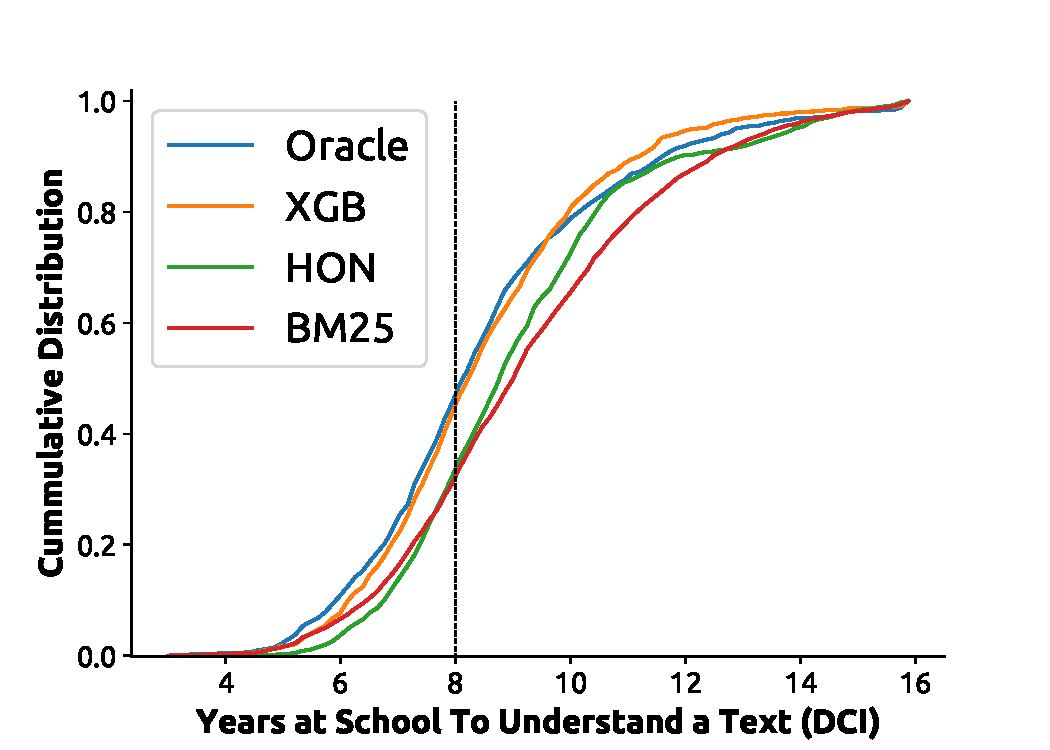
\includegraphics[width=.51\textwidth]{graphics/cumdist}
	%\vspace{-0.2cm}
	\caption{Distribution of Dale-Chall Index (DCI) of search results. DCI measures the years of schooling required to understand a document. The average US resident reads at or below an 8th grade level (dashed line) \cite{cowan04,wallace04,davis04,stossel12}, which is the level suggested by NIH for health information on the Web~\cite{clear94}. The distribution for HON is similar to that of the baseline used in this article (BM25). Our best method (XGB) re-ranks documents to provide more understandable results; its distribution is similar to that of an ``Oracle'' system.}
	\label{fig:dist}
\end{figure}




% =================================================================================================================================== %
% =================================================================================================================================== %
% =================================================================================================================================== %


\subsection{Related Work}

\label{sec:related}
Understandability refers to the ease of comprehension of the information presented to a user. Put in other words, health information is understandable ``when consumers of diverse backgrounds and varying levels of health literacy can process and explain key messages''~\cite{shoemaker2014development}. Often the terms understandability and readability are used interchangeably: we use readability to refer to formulae that estimate how easy is to understand a text, usually based on its words and sentences. We use understandability to refer to the broader concept of ease of understanding: this is affected by text readability (as increasing readability tends to improve understanding), but may also be influenced by how legible a text is and its layout, including e.g., the use of images to explain difficult concepts.

There is a large body of literature that has examined the understandability of Web health content when the information seeker is a member of the general public. For example, Becker reported that the majority of health Web sites are not well designed for the elderly~\cite{becker04}, while Stossel et al. found that  health education material on the Web is not written at an adequate reading level~\cite{stossel12}. Zheng and Yu have reported on the readability of electronic health records compared to Wikipedia pages related to diabetes and found that readability measures often do not align with user ratings of readability~\cite{zheng2017readability}. 
A common finding of these studies is that, in general, health content available on Web pages is often hard to understand by the general public; this includes content that is retrieved in top-ranked positions by current commercial search engines~\cite{graber99,fitzsimmons10,wiener13,patel13,meillier17}.

Previous Linguistics and Information Retrieval research has attempted to devise computational methods for the automatic estimation of text readability and understandability, and for the inclusion of these within search methods or their evaluation. Computational approaches to understandability estimations include (1) \textit{readability formulae}, which generally exploit word surface characteristics of the text, (2) \textit{machine learning} approaches, (3) matching with specialised \textit{dictionaries or terminologies}, often compiled with information about understandability difficulty.

Measures such as Coleman-Liau Index (CLI)~\cite{cli75}, Dale-Chall Index (DCI)~\cite{dale48} and Flesch Reading Easy (FRE)~\cite{flesch75}
belong to the first category. These measures generally rely on surface-level characteristics of text, such as characters, syllables and word counts~\cite{dubay04}. While these measures have been widely used in studies investigating the understandability of health content retrieved by search engines (e.g.,~\cite{becker04,graber99,fitzsimmons10,stossel12,wiener13,patel13,meillier17}), 
our preliminary work found that these measures are heavily affected by the methods used to extract text from the HTML source~\cite{palotti15}. We were able to identify specific settings of an HTML preprocessing pipeline that provided consistent estimates, but due to the lack of human assessments, we were not able to investigate how well each HTML preprocessing pipeline correlated with human assessments.
In this article, we revisited and extended this work in more detail, as we further investigated this problem by comparing the effect of HTML preprocessing on text understandability estimations in light of explicit human assessments. 

The use of machine learning to estimate understandability forms an alternative approach. Earlier research explored the use of statistical natural language processing and language modelling~\cite{liu04,collins05,heilman07} as well as linguistic factors, such as syntactic features or lexical cohesion~\cite{pitler08}. While we replicated here many of the features devised in these works, they focus on estimating readability of general English documents rather than medical ones. In the medical domain, Zeng et al. explored features such as word frequency in different medical corpora to estimate concept familiarity, which prompted the construction of the Consumer Health Vocabulary (CHV)~\cite{zeng05,zeng06,zeng08}.  

The actual use of CHV or other terminologies such as the Medical Subject Headings (MeSH) belongs to the third category of approaches. The CHV is a prominent medical vocabulary dedicated to mapping layperson vocabulary to technical terms~\cite{zeng06}. It attributes a score for each of its concepts with respect to their difficulty, with lower/higher scores for harder/easier concepts. Researchers have evaluated CHV in tasks such as document analysis~\cite{leroy08} and medical expertise prediction~\cite{palotti14}.
The hierarchy of MeSH was previously used in the literature to identify difficult concepts, assuming that a concept deep in the hierarchy is more difficult than a shallow one~\cite{yan11}. Other approaches combined vocabularies with word surface characteristics and syntactic features, like part of speech, into a unique readability measure~\cite{kim2007beyond}.

In this work, we investigated approaches to estimate understandability from each of these categories, including measure the influence of HTML preprocessing on automatic understandability methods and establish best practices. 

Some prior work has attempted to use understandability estimations for improving search results in consumer health search; as well as methods to evaluate retrieval systems that do account for understandability along with topical relevance. Palotti et al. have used learning to rank with standard retrieval features along with features based on readability formulae and medical lexical aspects to determine understandability~\cite{palotti2016ranking}. Van Doorn et al. have shown that learning a set of rankers that provide trade-offs across a number of relevance criteria, including readability/understandability, increases overall system effectiveness~\cite{van2016balancing}.
Zuccon and Koopman~\cite{zuccon14}, and later Zuccon~\cite{zuccon2016understandability}, have proposed and investigated a family of measures based on the gain-discount framework, where the gain of a document is influenced by both its topical relevance and its understandability. They showed that, although generally correlated, topical-relevance evaluation alone provides differing system rankings compared to understandability-biased evaluation measures. 
In this work, we further explored the development of retrieval methods that combine signals about topical relevance and understandability. 


\section*{Methods}
\label{sec:data}

\subsection*{Data Collection}

In this article, we investigated methods to estimate Web page understandability, including the effect HTML preprocessing pipelines and heuristics have, and their search effectiveness when employed within retrieval methods. To obtain both topical relevance and  understandability assessments, we used the data from the CLEF 2015 and 2016 eHealth collections. The CLEF eHealth initiative is a research community shared task aimed at creating resources for evaluating health search engines aimed at the general public.  Note, in the reminder of this article, we refer to topical relevance simply as relevance, when this does not cause confusion.

The CLEF 2015 collection contains 50 queries and 1,437 documents that have been assessed relevant by clinical experts and have an assessment for understandability~\cite{clef15}. Documents in this collection are a selected crawl of health Web sites, of which the majority are certified HON Web sites.
The CLEF 2016 collection contains 300 queries and 3,298 relevant documents that also have been assessed with respect to understandability~\cite{clef16}. Documents in this collection belong to the ClueWeb12 B13 corpus~\cite{clueweb12}, and thus are general English Web pages, not necessarily targeted to health topics, nor of a controlled quality (as are the HON certified pages). 
Understandability assessments were provided on a 5-point Likert scale for CLEF 2015, and on a $[0,100]$ range for CLEF 2016 (0 indicates the highest understandability). 

To support the investigation of methods to automatically estimate the understandability of Web pages, 
we further considered correlations between multiple human assessors (inter-assessor agreement). For CLEF 2015, we used the publicly available additional assessments made by unpaid medical students and health consumers collected by Palotti et al.~\cite{palotti16b} in a study of how medical expertise affects assessments. For CLEF 2016 we  collected understandability assessments for 100 documents. 
Three members of our research team, who did not author this article and are not medical experts, were recruited to provide the assessments (the correlation of these additional assessments and CLEF's ground-truth is examined further in this article).
The Relevation tool~\cite{koopman14} was used to assist with the assessments, mimicking the settings used in CLEF. 


\subsection*{Understandability Estimators}
\label{sec:proxies}

Several methods have been used to estimate the understandability of health Web pages, with the most popular methods (at least in the biomedical literature) being readability formulae based on surface level characteristics of the text. Next, we outline the categories of methods to estimate understandability used in this work; an overview is shown in Table~\ref{tab:doc_features}. Some of these features stem from common aspects used by readability measures, e.g., number of words longer than a set length in characters.

\begin{table*}[tb]
	\caption{Methods used to estimate understandability. $\star$: raw values were
		used. $\diamondsuit$: values normalised by number of words in a document
		were used. $\dagger$: values normalised by number of sentences in
		a document were used.}
	\label{tab:doc_features} \vspace{-10pt}
	\centering \resizebox{0.90\textwidth}{!}{ %
		\begin{tabular}{llccll}
			\toprule 
			\textbf{Cat.}  & \textbf{Method}  & \textbf{Cat.}  & \textbf{Method}  & \textbf{Cat.}  & \textbf{Method}\tabularnewline
			\midrule
			\multirow{8}{*}{\textbf{\makecell{RF}}}  & Automated Readability Index (ARI) \cite{ari67}  & \multirow{20}{*}{\textbf{\makecell{WFF}}}  & 25th percentil English Wikipedia  & \multirow{26}{*}{\textbf{\makecell{HF}}}  & \# of Abbr tags\tabularnewline
			& Coleman-Liau Index (CLI) \cite{cli75}  &  & 50th percentil English Wikipedia  &  & \# of A tags\tabularnewline
			& Dale-Chall Index (DCI) \cite{dale48}  &  & 75th percentil English Wikipedia  &  & \# of Blockquote tags\tabularnewline
			& Flesch-Kincaid Grade Level (FKGL) \cite{flesch75}  &  & Mean Rank English Wikip.  &  & \# of Bold tags\tabularnewline
			& Flesch Reading Ease (FRE) \cite{flesch75}  &  & Mean Rank English Wikip. - Includes OV  &  & \# of Cite tags\tabularnewline
			& Gunning Fog Index (GFI) \cite{gunning52}  &  & 25th percentil Medical Reddit  &  & \# of Div tags\tabularnewline
			& Lasbarhetsindex (LIX) \cite{lix}  &  & 50th percentil Medical Reddit  &  & \# of Forms tags\tabularnewline
			& Simple Measure of Gobbledygook (SMOG) \cite{smog69}  &  & 75th percentil Medical Reddit  &  & \# of H1 tags\tabularnewline
			\cline{1-2}
			\multirow{10}{*}{\textbf{\makecell{CRF}}}  & \# of Characters $^{\star\diamondsuit\dagger}$  &  & Mean Rank Medical Reddit  &  & \# of H2 tags\tabularnewline
			& \# of Words $^{\star\dagger}$  &  & Mean Rank Medical Reddit - Includes OV  &  & \# of H3 tags\tabularnewline
			& \# of Sentences {$^{\star\diamondsuit}$}  &  & 25th percentil Pubmed  &  & \# of H4 tags\tabularnewline
			& \# of Difficult Words (Dale-Chall list \cite{dale48}) $^{\star\diamondsuit\dagger}$  &  & 50th percentil Pubmed  &  & \# of H5 tags\tabularnewline
			& \# of Words Longer than 4 chars $^{\star\diamondsuit\dagger}$  &  & 75th percentil Pubmed  &  & \# of H6 tags\tabularnewline
			& \# of Words Longer than 6 chars $^{\star\diamondsuit\dagger}$  &  & Mean Rank Pubmed  &  & \# of Hs (any H above)\tabularnewline
			& \# of Words Longer than 10 chars $^{\star\diamondsuit\dagger}$  &  & Mean Rank Pubmed - Includes OV  &  & \# of Img tags\tabularnewline
			& \# of Words Longer than 13 chars $^{\star\diamondsuit\dagger}$  &  & 25th p. Wikipedia+Reddit+Pubmed  &  & \# of Input tags\tabularnewline
			& \# of Number of Syllables $^{\star\diamondsuit\dagger}$  &  & 50th p. Wikipedia+Reddit+Pubmed  &  & \# of Link tags\tabularnewline
			& \# of Polysyllable Words (\textgreater{}3 Syllables) $^{\star\diamondsuit\dagger}$  &  & 75th p. Wikipedia+Reddit+Pubmed  &  & \# of DL tags\tabularnewline
			\cline{1-2}
			\multirow{20}{*}{\textbf{\makecell{NLF}}}  & \# of Entities $^{\star\diamondsuit\dagger}$  &  & Mean R. Wiki.+Reddit+Pubmed  &  & \# of UL tags\tabularnewline
			& \# of verbs $^{\star\diamondsuit\dagger}$  &  & Mean R. Wiki.+Reddit+Pubmed - w. OV  &  & \# of OL tags\tabularnewline
			\cline{3-4} 
			& \# of nouns $^{\star\diamondsuit\dagger}$  & \multirow{6}{*}{\textbf{GMV}}  & \# of Words with Medical Prefix $^{\star\diamondsuit\dagger}$  &  & \# of List (DL + UL + OL)\tabularnewline
			& \# of pronouns $^{\star\diamondsuit\dagger}$  &  & \# of Words with Medical Suffix $^{\star\diamondsuit\dagger}$  &  & \# of Q tags\tabularnewline
			& \# of adjectives $^{\star\diamondsuit\dagger}$  &  & \# of Acronyms $^{\star\diamondsuit\dagger}$  &  & \# of Scripts tags\tabularnewline
			& \# of adverbs $^{\star\diamondsuit\dagger}$  &  & \# of ICD Concepts $^{\star\diamondsuit\dagger}$  &  & \# of Spans tags\tabularnewline
			& \# of adpositions $^{\star\diamondsuit\dagger}$  &  & \# of Drugbank $^{\star\diamondsuit\dagger}$  &  & \# of Table tags\tabularnewline
			& \# of conjunctions $^{\star\diamondsuit\dagger}$  &  & \# of Words in medical dict. (OpenMedSpel) $^{\star\diamondsuit\dagger}$  &  & \# of P tags\tabularnewline
			\cline{3-6}
			& \# of determiners $^{\star\diamondsuit\dagger}$  & \multirow{6}{*}{\textbf{\makecell{CMV}}}  & CHV Mean Score for all Concepts $^{\star\diamondsuit\dagger}$  & \multirow{6}{*}{\textbf{MLR}}  & Linear Regressor\tabularnewline
			& \# of cardinal numbers $^{\star\diamondsuit\dagger}$  &  & \# of CHV Concepts $^{\star\diamondsuit\dagger}$  &  & Multi-layer Perceptron Regressor\tabularnewline
			& \# of particles or other function words $^{\star\diamondsuit\dagger}$  &  & CHV Mean Score for Symptom Concepts $^{\star\diamondsuit\dagger}$  &  & Random Forest Regressor\tabularnewline
			& \# of other POS (foreign words, typos) $^{\star\diamondsuit\dagger}$  &  & \# of CHV Symptom Concepts $^{\star\diamondsuit\dagger}$  &  & Support Vector Machine Regressor\tabularnewline
			& \# of punctuation $^{\star\diamondsuit\dagger}$  &  & CHV Mean Score for Disease Concepts $^{\star\diamondsuit\dagger}$  &  & Gradient Boosting Regressor\tabularnewline
			& Height of part-of-speech parser tree $^{\star\diamondsuit\dagger}$  &  & \# of CHV Disease Concepts $^{\star\diamondsuit\dagger}$  &  & Logistic Regression\tabularnewline
			\cline{3-6} 
			& \# of Stopwords $^{\star\diamondsuit\dagger}$  & \multirow{6}{*}{\textbf{\makecell{EMV}}}  & \# of MeSH Concepts $^{\star\diamondsuit\dagger}$  & \multirow{5}{*}{\textbf{MLC}}  & Multi-layer Perceptron Classifier\tabularnewline
			& \# of words not found in Aspell Eng. dict. $^{\star\diamondsuit\dagger}$ &  & Average Tree of MeSH Concepts $^{\star\diamondsuit\dagger}$  &  & Random Forest Classifier\tabularnewline
			& Positive Words $^{\star\diamondsuit\dagger}$  &  & \# of MeSH Symptom Concepts $^{\star\diamondsuit\dagger}$  &  & Support Vector Machine Classifier\tabularnewline
			& Negative Words $^{\star\diamondsuit\dagger}$ &  & Average Tree of MeSH Symptom Concepts $^{\star\diamondsuit\dagger}$  &  & Multinomial Naive Bayes\tabularnewline
			& Neutral Words $^{\star\diamondsuit\dagger}$  &  & \# of MeSH Disease Concepts $^{\star\diamondsuit\dagger}$  &  & Gradient Boosting Classifier\tabularnewline
			&  &  & Average Tree of MeSH Disease Concepts $^{\star\diamondsuit\dagger}$  &  & \tabularnewline
			\bottomrule 
	\end{tabular}} \vspace{-12pt}
	
\end{table*}


\textit{Traditional Readability Formulae (RF):}
These include the most popular readability formulae~\cite{cli75,dale48,flesch75}, as well as other, less popular ones~\cite{ari67,gunning52,lix,smog69}. A full list is provided in surveys by Collins-Thompson \cite{collins2014computational} and Dubay~\cite{dubay04}.

\textit{Raw Components of Readability Formulae (CRF):}
These are formed by the ``building blocks'' used in the traditional readability formulae. Examples include the average number of characters per word and the average number of syllables in a sentence. Words are divided into syllables using the Python package Pyphen~\cite{pyphen}.

\textit{General Medical Vocabularies (GMV):}
These include methods that count the number of words with a medical prefix or suffix, i.e. beginning or ending with Latin or Greek particles (e.g., amni-, angi-, algia-, arteri-), and text strings included in lists of acronyms or in medical vocabularies such as the International Statistical Classification of Diseases and Related Health Problems (ICD), Drugbank and the OpenMedSpel dictionary~\cite{openmedspel}. An acronym list from the ADAM database~\cite{zhou2006} was used. Methods in this category were matched with documents using simple keyword matching. 

\textit{Consumer Medical Vocabulary (CMV):}
The popular MetaMap \cite{aronson10} tool was used to map the text content of Web pages to entries in  CHV~\cite{zeng06}.
We used the MetaMap semantic types to retain only concepts identified as symptoms or diseases. Similar approaches have been commonly used in the literature (e.g.,~\cite{pang16,agrafiotesA16,palotti16,yates13}).

\textit{Expert Medical Vocabulary (EMV):}
Similarly to the CHV features, we used MetaMap to convert the content of Web pages into MeSH entities, studying symptom and disease concepts separately. 

\textit{Natural Language Features (NLF):}
These included commonly used natural language heuristics such as the ratio of part-of-speech (POS) classes, the height of the POS parser tree, the number of entities in the text, 
the sentiment polarity~\cite{pang08} and the ratio of words found in English vocabularies. The Python package NLTK~\cite{nltk} was employed for sentiment analysis, POS tagging and entity recognition. The GNU Aspell~\cite{aspell} dictionary was used as a standard English vocabulary and a stop word list was built by merging those of Indri~\cite{indri} and Terrier~\cite{terrier}. 
Discourse features, such as the distribution of POS classes and density of entity in a text, were previously studied in the task of understandability prediction~\cite{feng10} and found superior to complex features such as entity co-reference and entity grid~\cite{barzilay08}. To the best of our knowledge, sentiment polarity was never investigated in this task. Our intuition is that the content produced by laypeople in patient forums or blogs (easy-to-read) is potentially more emotional than scientific publications (hard-to-read).

\textit{HTML Features (HF):}
These include the identification of a large number of HTML tags, which were extracted with the Python library BeautifulSoup~\cite{bs4}. The intuition for these features is that Web pages with many images and tables may explain and summarise health content better, thus providing more understandable content to the general public. 

\textit{Word Frequency Features (WFF):}
Generally speaking, common and known words are usually frequent words, while unknown and obscure words are generally rare. This idea is implemented in readability formulae such as the DCI, which uses a list of common words and counts the number of words that fall outside this list (complex words)~\cite{dale48} and has shown success in other recent approaches~\cite{elhadad06,wu15}.
We extended these observations by studying corpus-wide word frequencies. 
Three corpora were analysed to extract word frequencies:

\begin{itemize}[leftmargin=*]
	\item \underline{Medical Reddit:} Reddit~\cite{reddit} is a Web forum with a sizeable user community which is responsible for generating and moderating its content. This forum is intensively used for health purposes: for example in the Reddit community AskDocs~\cite{redditaskdocs}, licensed nurses and doctors (subject to user identity verification) advise help seekers free of charge. We selected six of such communities (medical, AskDocs, AskDoctorSmeeee, Health, WomensHealth, Mens\_Health) and downloaded all user interactions available until September 1st 2017 using the Python library PRAW~\cite{redditapi}. In total 43,019 discussions were collected.
	
	\item \underline{Medical English Wikipedia:} after obtaining a recent Wikipedia dump~\cite{wikipedia} (May 1st 2017), we filtered articles to only those containing an Infobox in which at least one of the following words appeared as a property: ICD10, ICD9, DiseasesDB, MeSH, MeSHID, MeshName, MeshNumber, GeneReviewsName, Orphanet, eMedicine, MedlinePlus, drug\_name, Drugs.com, DailyMedID, LOINC. A Wikipedia infobox is a structured template that appears on the right of Wikipedia pages summarising key aspects of articles. 
	This process followed the method by Soldaini et al.~\cite{soldaini15}, which favours precision over recall when identifying a health-related article. This resulted in a collection of 11,868 articles. 
	
	\item \underline{PubMed Central:} PubMed Central~\cite{pubmed} is an online  database of biomedical literature. We used the collection distributed for the TREC 2014 and 2015 Clinical Decision Support Track~\cite{roberts16,trec15}, consisting of 733,191 articles. 
	
\end{itemize}

A summary of the statistics of the corpora is reported in Table~\ref{tab:collection_stats}. 
We modelled word frequencies in a corpus in a straightforward manner: we sorted the word frequencies and normalised word rankings such that values close to 100 are attributed to common words and values close to 0 to rare words. Then we replace each word in a document by a number ranging from 0 to 100 which represents the frequency of that word in the corpus. 
Finally, we extract features based on the word frequency distribution for that document. For example, in order to calculate the feature \textit{25th percentil English Wikipedia} of a document, we need first to extract the frequency of each word in the Wikipedia corpus for that document and then extract the 25th percentil of the frequency distribution of that document. 
Unless explicitly stated otherwise, we ignored out of vocabulary (OV) words in the corpus.

\begin{table*}[!tb]
	\centering    
	\caption{Statistics for the corpora used as background models for understandability estimations.}
	%\vspace{-0.3cm}
	\label{tab:collection_stats}
	\resizebox{0.6\textwidth}{!}{
		\begin{tabular}{cccc}
			\toprule 
			\textbf{Statistic} & \textbf{Medical Wikipedia} & \textbf{Medical Reddit} & \textbf{PubMed Central}\tabularnewline
			\midrule 
			\textbf{Number of Docs.} & 11,868 & 43,019 & 733,191\tabularnewline
			\textbf{Number of Words} & 10,655,572 & 11,978,447 & 144,024,976\tabularnewline
			\textbf{Number of Unique Words} & 467,650 & 317,106 & 2,933,167\tabularnewline
			\textbf{Avg. Words per Doc.} & 898.90 $\pm$ 1351.76 & 278.45 $\pm$ 359.70  & 227.22 $\pm$ 270.44 \tabularnewline
			\textbf{Avg. Char per Doc.} & 5,107.81 $\pm$ 7,618.57  & 1,258.44 $\pm$ 1,659.96  & 1,309.11 $\pm$ 1,447.31 \tabularnewline
			\textbf{Avg. Char per Word} & 5.68 $\pm$ 3.75  & 4.52 $\pm$ 3.52 &  5.76 $\pm$ 3.51 \tabularnewline
			\bottomrule
		\end{tabular}
	} % End of resizebox
	%\vspace{-8pt}
\end{table*}


\textit{Machine Learning on Text - Regressors (MLR) and Classifiers (MLC):} These include machine learning methods for estimating Web page understandability. While Collins-Thompson highlighted the promise of estimating understandability using machine learning methods, a challenge is identifying the background corpus to be used for training~\cite{collins2014computational}. To this aim, we used the three corpora detailed above, and assumed understandability labels according to the expected difficulty of documents in these collections:

\begin{itemize}[leftmargin=*]
    \item Medical Reddit (label 1): Documents in this corpus are expected to be written in a colloquial style, and thus the easiest to understand. All the conversations are in fact explicitly directed to assist inexpert health consumers;
	\item Medical English Wikipedia (label 2): Documents in this corpus are expected to be less formal than scientific articles, but more formal than a Web forum like Reddit, thus somewhat more difficult to understand;
	\item PubMed Central (label 3): Documents in this corpus are expected to be written in a highly formal style, as the target audience are physicians and biomedical researchers.
\end{itemize}

Based on the labels of each class above, models were learnt using all documents from these corpora after features were extracted using Latent Semantic Analysis (LSA) with 10 dimensions (this number of dimensions was chosen based on preliminary experiments with the Random Forest algorithm; we leave as future work a detailed study on the impact of different number of dimensions on other machine learning algorithms). We modelled a classification task as well as a regression task using these corpora. Thus, after applying the same LSA transformation to test documents from CLEF, a continuous score was assigned to each document by a regressor, while each classifier assigned the documents to one of the three classes. 


\subsection*{Preprocessing Pipelines and Heuristics}
\label{sec:pipelines}

As part of our study, we investigated the influence that the preprocessing of Web pages has on the estimation of understandability computed using the methods described above.
We did so by comparing the combination of a number of preprocessing pipelines, heuristics, and understandability estimation methods with human assessments of Web page understandability. 
Our experiments extended those by Palotti et al.~\cite{palotti15} and provided a much more thorough analysis, as they only evaluated surface level readability formulae and did not compare their results against human assessments. 

To extract the content of a Web page from the HTML source we tested: BeautifulSoup~\cite{bs4} (\textit{Naive}), which just naively removes HTML tags, Boilerpipe~\cite{kohlschutter10} (\textit{Boi}) and Justext~\cite{jan11} (\textit{Jst}), which eliminates boilerplate text together with HTML tags. 
Palotti et al.'s data analysis highlighted that the text in HTML fields like titles, menus, tables and lists often missed a correct punctuation mark and thus the text extracted from them could be interpreted as many short sentences or few very long sentences, depending on whether a period was forced at the end of fields/sentences. We thus implemented the same two heuristics devised by Palotti et al. to deal with this: \textit{ForcePeriod (FP)} and \textit{DoNotForcePeriod (DNFP)}. 
If a punctuation mark is found at the end of a field/sentence, it is kept as it is. However, if no punctuation mark is not found at the end of a field/sentence, the FP heuristic forces the insertion of a period at the end of that extracted HTML field, while the DNFP does not.

\subsection*{Integrating Understandability into Retrieval}
\label{sec:method_ltr}

We then investigated how understandability estimations can be integrated into retrieval methods to increase the quality of search results.
Specifically, we considered three retrieval methods of differing quality for the initial retrieval. These included the best two runs submitted to each CLEF task, and a plain BM25 baseline (default Terrier parameters: $b=0.75$ and $k_1=1.2$). BM25 is a probabilistic term weighting scheme commonly used in information retrieval and is defined with respect to the frequency of a term in a document, the collection frequency of that term, and the ratio between the length of the document and the average document length. As understandability estimators we used the eXtreme Gradient Boosting (XGB) regressor~\cite{chen16}, as well as SMOG for CLEF 2015 and DCI for CLEF 2016. 
These were selected as they were the best performing readability formulae and machine learning method for each collection (details in the evaluation of understandability estimators in the Results section).
Note that for XGB, for assessed documents we used 10-fold cross validation, training XGB on 90\% of the data, and used its predictions for the remaining 10\%. For unassessed documents, we trained XGB on all assessed data and applied this model to generate predictions. Different machine learning methods and feature selection schemes were experimented with; results are available in the appendix. XGB was selected because its results were the best, although other methods followed similar trends \todo{15 - Very vague. -- say explicitly which methods and which trends}.


To integrate understandability estimators into the retrieval process, we first investigated \textit{re-ranking} search results retrieved by the initial runs purely based on the understandability estimations. 
If all the search results from a run were to be considered, then such a re-ranking method may place at early ranks Web pages highly likely to be understandable, but possibly less likely to be topically relevant. To balance relevance and understandability, we only re-ranked the first $k$ documents. We explored rank cut-offs $k = 15, 20, 50$. Because evaluation was performed with respect to the first $n=10$ rank positions, the setting $k=15$ provided a conservative re-ranking of search results, while, $k=50$ provided a less conservative re-ranking approach.

As an alternative to the previous two-step ranking strategy for combining topical relevance and understandability, we explored the \textit{fusion} of two search results lists separately obtained for relevance and understandability. For this, we used the Reciprocal Rank Fusion (RRF) method~\cite{cormack09}, which was shown effective for combining two lists of search results based on their documents' \textit{ranks}, rather than scores. This approach was selected above score-based fusion methods
because the distribution of relevance scores for the retrieved documents different sensibly (both in magnitude and spread) with that of understandability scores: in such a case score-based fusion is not appropriate. 
For relevance, we used, separately, the three methods used for re-ranking (ECNU~\cite{song15} and KISTI~\cite{oh15} for CLEF2015, GUIR~\cite{soldaini16} and ECNU~\cite{song16} for CLEF 2016, and BM25 for both collections). For understandability, we used, separately, the estimations from SMOG/DCI and XGB. Also for this approach, we studied limiting the ranking of
results to be considered by the methods across the cut-offs $k=15, 20, 50$. 

%\begin{table}[!t]
%	\centering
%	\caption{Learning to rank (LTR) settings. }
%	\label{tab:ltr}
%	\resizebox{0.45\textwidth}{!}{
%		\begin{tabular}{l|l|l}
%			\toprule 
%			Name & Feature Set & Labelling Function\tabularnewline
%			\midrule 
%			LTR 1 & IR features & F(R,U) = $R$\tabularnewline
%			LTR 2 & IR + Unders. features & F(R,U) = $R$ \tabularnewline
%			LTR 3 & IR + Unders. features & F(R,U) = $R \times (100 - U)/100$ \tabularnewline
%			LTR 4 & IR + Unders. features & F(R,U) = $\begin{cases} R & \text{if } U \le 40\\ 0 & \text{otherwise}  \end{cases}$ \tabularnewline
%			LTR 5 & IR + Unders. features & F(R,U) = $\begin{cases} 2 \times R & \text{if } U \le 40\\ R & \text{otherwise}  \end{cases}$\tabularnewline
%			\bottomrule
%		\end{tabular}
%	}% end resizebox
%\end{table}

\begin{table}[!t]
    \centering \caption{Learning to rank settings. }
    \label{tab:ltr} \resizebox{.99\textwidth}{!}{ %
        \begin{tabular}{llll}
            \toprule 
            \multirow{2}{*}{\textbf{Name}} & \multirow{2}{*}{\textbf{Explanation}} & \multicolumn{2}{l}{\textbf{Labeling Function}}\tabularnewline
            \cmidrule{3-4} 
            &  & \textbf{CLEF 2015} & \textbf{CLEF 2016}\tabularnewline
            \midrule 
            LTR 1  & Builds a model \textit{only} on the topicality labels w. IR features & F(R,U) = $R$ & F(R,U) = $R$\tabularnewline
            LTR 2  & Builds a model \textit{only} on the topicality labels w. IR and Unders. features & F(R,U) = $R$  & F(R,U) = $R$ \tabularnewline
            LTR 3  & Directly combines unders. and topicality labels. Uses IR and unders. features & F(R,U) = $R\times U/3.$  & F(R,U) = $R\times(100-U)/100$ \tabularnewline
            LTR 4  & Builds the model \textit{only} on easy-to-read docs. Uses IR and unders. features & F(R,U) = $\begin{cases} R & \text{if }U\geq2\\ 0 & \text{otherwise} \end{cases}$  & F(R,U) = $\begin{cases} R & \text{if }U\le40\\ 0 & \text{otherwise} \end{cases}$ \tabularnewline
                LTR 5  & Boosts easy-to-read documents. Uses IR and unders. features & F(R,U) = $\begin{cases} 2\times R & \text{if }U\geq2\\ R & \text{otherwise} \end{cases}$ & F(R,U) = $\begin{cases} 2\times R & \text{if }U\le40\\ R & \text{otherwise}
        \end{cases}$\tabularnewline
    \bottomrule
\end{tabular}
}% end resizebox
\end{table}

Finally, we considered a third alternative to combine relevance and understandability: using \textit{learning to rank} with features derived from retrieval methods (IR features) and understandability estimators.
With the CLEF 2015 and 2016 collections, we explored five combinations of label attribution and feature sets, maintaining the same pairwise learning to rank algorithm based on tree boosting (XGB).
These combinations are listed in Table~\ref{tab:ltr}, with $R$ being the relevance of documents and $U$ their understandability estimation. While the definitions of LTR 1 and 2 are straightforward, the other methods deserve some further explanation. In LTR 3, a penalty was proportionally assigned to documents according to their understandability score $U$. For example, for CLEF 2016, a document with understandability $U=0$ received no penalty, as 0 was the easiest level of understanding, while another with understandability 50 received a 50\% penalty, meaning that its relevance score was halved. LTR 4 and 5 were based on a fixed threshold applied to the understandability score: if the score was higher than the threshold ($U=2$ for CLEF 2015 and $U=40$ for CLEF 2016), then the original relevance score (for LTR 4) or a boosted value (for LTR 5) was assigned to the corresponding document. We used the thresholds $U=2$ for CLEF 2015 and $U=40$ for CLEF 2016 based on the distribution of
understandability assessments and the semantic of understandability labels~\cite{clef15,clef16}.


\subsection*{Evaluation Measures}

In the experiments, we used Pearson, Kendall and Spearman correlations to compare the understandability assessments of human assessors with estimations obtained by the considered automated approaches, under all combinations of pipelines and heuristics. Pearson correlation is used to calculate the strength of the linear relationship between two variables, while Kendall and Spearman measure the rank correlations between the variables. We opted to report all three correlation coefficients to allow for a thorough comparison to other work, as they are equally used in the literature. 

For the retrieval experiments \todo{5 - Again, difficult to follow without knowing what the experiments are. I think especially difficult for people outside IR.}, we used evaluation measures that rely on both (topical) relevance and understandability. 
The uRBP measure~\cite{zuccon2016understandability} extends rank biased precision (RBP) to situations where multiple relevance dimensions are used. The measure is formulated as $uRBP(\rho) = (1 - \rho) \sum_{k=1}^{K} \rho^{k-1} r(d@k) u(d@k)$, where $r(d@k)$ is the gain for retrieving a relevant document at rank $k$ and $u(d@k)$ is the gain for retrieving a document of a certain understandability at rank $k$; $\rho$ is the RBP persistence parameter. This measure was an official evaluation measure used in CLEF (we also set $\rho=0.8$). 

A drawback of uRBP is that relevance and understandability are combined into a unique evaluation score, thus making it difficult to interpret whether improvements are due to more understandable or more topical documents being retrieved. To overcome this, we first separately calculated an RBP value for relevance and another for understandability, and then combined them into a unique effectiveness measure:

\begin{itemize}[leftmargin=*]
	\item $RBP_r@n(\rho)$: uses the relevance assessments for the top $n$ search results (i.e. this is the common RBP). We regarded a document as topically relevant if assessed as somewhat relevant or highly relevant.
	
    \item $RBP_u@n(\rho)$: uses the understandability assessments for the top $n$ search results. We regarded a document as understandable (1) for CLEF 2015 if assessed easy or somewhat easy to understand; (2) for CLEF 2016 if its assessed understandability score was smaller than a threshold $U$. We used $U=40$, based on the distribution of understandability assessments. Assessors were presented with a slider for understandability assessment and $U=50$ was labeled as average understandability. This created a bi-modal distribution of understandability assessments with $U=40$ being a good upper limit for easy-to-read documents. The understandability distribution can be found in the appendix.
	
	\item $H_{RBP}@n(\rho) = 2 \times \frac{RBP_r@n \times RBP_u@n}{RBP_r@n + RBP_u@n}$: combines the previous two RBP values into a unique measurement using the harmonic mean (in the same fashion that the $F_1$ measure combines recall and precision).
\end{itemize}

\noindent For all measures, we set $n=10$ because shallow pools were used in CLEF along with measures that focused on the top 10 search results (including $RBP_r@10$). Shallow pools refer to the selection of a limited number of documents to be assessed for relevance, among the documents retrieved at the top ranks by a search engine.

Along with these measures of search effectiveness, we also recorded the number of unassessed documents, the RBP residuals,  $RBP^*_r@10$, $RBP^*_u@10$ and $H_{RBP}^*$, i.e. the corresponding measures calculated by ignoring unassessed documents. These latter measures implement the condensed measures approach proposed by Sakai as a way to deal with unassessed documents~\cite{sakai2007alternatives}. We did this to minimise pool bias since the pools built in CLEF were of limited size, and the investigated methods retrieved a substantial number of unassessed documents. Pool bias refers to the possible bias in the evaluation towards systems that have contributed documents to the assessment pool: these erroneously receive higher evaluation scores compared to systems that did not contribute to the pool (i.e. that were not sampled to create the set of documents to be judged for relevance). 



\section*{Results}


In order to keep this article  succinct, in the following we only report a subset of the results. The remaining results (which show similar trends to those reported here) are made available in the appendix material  for completeness.  \textit{All data and code will be shared on GitHub upon acceptance.}
%\url{https://sites.google.com/view/understandabilityontheweb/}.

\subsection*{Evaluation of understandability estimators}
\label{sec:beyond_readability}


\begin{table*}[t]
	\centering    
	\caption{Methods with the highest correlation per category. Bold is used to highlight the best result of each group.}
	%\vspace{-10pt}
	\label{tab:top_corr_metrics}
	\resizebox{.95\textwidth}{!}{ %%%%
		\begin{tabular}{l|ccccc||ccccc}
			\toprule 
			\multirow{2}{*}{\textbf{Cat.} } & \multicolumn{5}{c}{\textbf{CLEF 2015}} & \multicolumn{5}{c}{\textbf{CLEF 2016}}\tabularnewline
			\cmidrule{2-11} 
			& \textbf{Method}  & \textbf{Preproc.}  & \textbf{Pears.}  & \textbf{Spear.}  & \textbf{Kend.} & \textbf{Method}  & \textbf{Preproc.}  & \textbf{Pears.}  & \textbf{Spear.}  & \textbf{Kend.}\tabularnewline
			\midrule 
			\multirow{2}{*}{\textbf{RF}} & \multirow{2}{*}{SMOG Index } & \multirow{2}{*}{Jst NFP } & \multirow{2}{*}{\textbf{.438} } & \multirow{2}{*}{\textbf{.388} } & \multirow{2}{*}{\textbf{.286}} & \multirow{2}{*}{Dale-Chall Index } & Jst FP  & \textbf{.439}  & .381  & .264\tabularnewline
			&  &  &  &  &  &  & Boi FP  & .437  & \textbf{.382}  & \textbf{.264}\tabularnewline
			\midrule 
			\multirow{2}{*}{\textbf{CRF}} & Avg. Num. of Polysyl. Words per Word  & Jst FP  & \textbf{.429}  & .364  & .268 & \multirow{2}{*}{Avg. Difficult Words Per Word } & \multirow{2}{*}{Boi FP } & \multirow{2}{*}{\textbf{.431} } & \multirow{2}{*}{\textbf{.379} } & \multirow{2}{*}{\textbf{.262}}\tabularnewline
			& Avg. N. of Polysyl. Words per Sentence  & Jst NFP  & .192  & \textbf{.388}  & \textbf{.286} &  &  &  &  & \tabularnewline
			\midrule 
			\multirow{2}{*}{\textbf{GMV}}  & Avg. N. Medical Prefixes per Word  & \multirow{2}{*}{Naive FP} & \textbf{.314}  & .312  & .229 & Avg. Prefixes per Sentence  & Jst FP  & \textbf{.263}  & .242  & .164\tabularnewline
			& Number of Medical Prefixes  &  & .131  & \textbf{.368}  & \textbf{.272} & ICD Concepts Per Sentence  & Jst NFP  & .014  & \textbf{.253}  & \textbf{.172}\tabularnewline
			\midrule 
			\multirow{2}{*}{\textbf{CMV}} & \multirow{2}{*}{CHV Mean Score for all Concepts } & \multirow{2}{*}{Naive FP } & \multirow{2}{*}{\textbf{.371} } & \multirow{2}{*}{\textbf{.314} } & \multirow{2}{*}{\textbf{.228}} & CHV Mean Score for all Concepts  & Jst FP  & \textbf{.329}  & .313  & .216\tabularnewline
			&  &  &  &  &  & CHV Mean Score for all Concepts  & Boi FP  & .329  & \textbf{.325}  & \textbf{.224}\tabularnewline
			\midrule 
			\multirow{2}{*}{\textbf{EMV}} & \multirow{2}{*}{Number of MeSH Concepts } & \multirow{2}{*}{Naive FP } & \multirow{2}{*}{\textbf{.227} } & \multirow{2}{*}{\textbf{.249} } & \multirow{2}{*}{\textbf{.178}} & Number of MeSH Concepts  & \multirow{2}{*}{Boi NFP } & \textbf{.201}  & .166  & .113\tabularnewline
			&  &  &  &  &  & Number of MeSH Disease Concepts  &  & .179  & \textbf{.192}  & \textbf{.132}\tabularnewline
			\midrule 
			\multirow{2}{*}{\textbf{NLF}} & N. of words not found in Aspell Dict.  & Jst NFP  & \textbf{.351}  & .276  & .203 & Avg. Stopword Per Word  & \multirow{2}{*}{Boi FP } & \textbf{.344}  & .312  & .213\tabularnewline
			& Number of Pronouns per Word  & Naive FP  & .271  & \textbf{.441}  & \textbf{.325} & Number of Pronouns  &  & .341  & \textbf{.364}  & \textbf{.252}\tabularnewline
			\midrule 
			\multirow{2}{*}{\textbf{HF}} & \multirow{2}{*}{Number of P Tags } & \multirow{2}{*}{None } & \multirow{2}{*}{\textbf{.219} } & \multirow{2}{*}{\textbf{.196} } & \multirow{2}{*}{\textbf{.142}} & Number of Lists  & \multirow{2}{*}{None} & \textbf{.114}  & .021  & .015\tabularnewline
			&  &  &  &  &  & Number of P Tags  &  & .110  & \textbf{.123}  & \textbf{.084}\tabularnewline
			\midrule 
            \multirow{2}{*}{\textbf{WFF}} & Mean Rank Medical Reddit - Includes OV  & Jst NFP  & \textbf{.435}  & .277  & .197 & Mean Rank Medical Reddit  & Boi NFP  & \textbf{.387}  & .312  & .214\tabularnewline
			& 25th percentil Pubmed  & Jst NFP  & .330  & \textbf{.347}  & \textbf{.256} & 50th percentil Medical Reddit  & Jst NFP  & .351  & \textbf{.315}  & \textbf{.216}\tabularnewline
			\midrule 
			\multirow{2}{*}{\textbf{MLR}} & eXtreme Gradient Boosting (XGB) Regressor  & Boi NFP  & \textbf{.602}  & .394  & .287 & eXtreme Gradient Boosting (XGB) Regressor  & Jst NFP  & \textbf{.454}  & \textbf{.373}  & .258\tabularnewline
			& eXtreme Gradient Boosting (XGB) Regressor  & Jst FP  & .565  & \textbf{.438}  & \textbf{.324} & Random Forest Regressor  & Boi NFP  & .389  & .355  & \textbf{.264}\tabularnewline
			\midrule 
			\textbf{MLC} & Multinomial Naive Bayes  & Naive FP  & \textbf{.573}  & \textbf{.477}  & \textbf{.416} & Multinomial Naive Bayes  & Jst FP  & \textbf{.461}  & \textbf{.391}  & \textbf{.318}\tabularnewline
			\bottomrule
		\end{tabular}
	} %%%%% ---- 
\end{table*}


Using the CLEF eHealth 2015 and 2016 collections, we studied the correlations of methods to estimate Web page understandability (Table~\ref{tab:doc_features}), compared with human assessments. For each category of understandability estimation, Table~\ref{tab:top_corr_metrics} reports the methods with highest Pearson, Spearman or Kendall correlations. For each method, we used the best preprocessing settings; a study of the impact of preprocessing is reported in the next subsection.

Overall, Spearman and Kendall correlations obtained similar results (in terms of which methods exhibited the highest correlations): this was expected as, unlike Pearson, they are both rank-based correlations.

For traditional readability measures, SMOG had the highest correlations for CLEF 2015 and DCI for CLEF 2016, regardless of correlation measure. These results resonate with those obtained for the category of raw components of readability formulae. 
In fact, the polysyllable words measure, which is the main feature used in SMOG, had the highest correlation for CLEF 2015 among methods in this category. Similarly, the number of difficult words, which is the main feature used in DCI, had the highest correlation for CLEF 2016 among methods in this category.

When examining the expert vocabulary category, we found that the number of MeSH concepts obtained the highest correlations with human assessments; however, its correlations were substantially lower than those achieved by the best method from the consumer medical vocabularies category, i.e. the scores of CHV concepts. For the natural language category, we found that the number of pronouns, the number of stop words and the number of out of vocabulary (OV) words had the highest correlations -- and these were even higher than those obtained with MeSH and CHV based methods. In turn, the methods that obtained the highest correlations among the HTML category (counts of P tags and list tags) exhibited overall the lowest correlations compared to methods in the other categories. P tags are used to create paragraphs in a Web page, being thus a rough proxy for text length. 
Among methods in the word frequency category, the use of Medical Reddit (but also of PubMed) showed the highest correlations, and these were comparable to those obtained by the readability formulae. 

Finally, regressors and classifiers exhibited the highest correlations amongst all methods: in this  category, the  eXtreme Gradient Boosting (XGB) regressor and the multinomial Naive Bayes best correlated with human assessments. 

\subsection*{Evaluation of Preprocessing Pipelines and Heuristics}
\label{sec:which_preprocessing}

Results from experiments with different preprocessing pipelines and heuristics are shown in Figure~\ref{fig:boxplot_corr_docs} (top: CLEF 2015; bottom: CLEF 2016). 
For each category of methods and combination of preprocessing and heuristics, we report their variability in terms of Spearman rank correlation with human assessments. Results for Pearson and Kendall correlations are reported in the appendix, but showed similar trends. 
We further report the summary results across all understandability assessment methods and sentence-ending heuristics for each of the preprocessing pipelines. 
Finally, we also report the inter-assessor correlation (last box) when multiple assessors provided judgements about the understandability of Web pages. % (details about this data in Section~\ref{sec:data}). 
This provides an indication of the range of variability and subjectiveness when assessing understandability, along with the highest correlation we measured between human assessors. 

\begin{figure*}[h!]
	\centering
	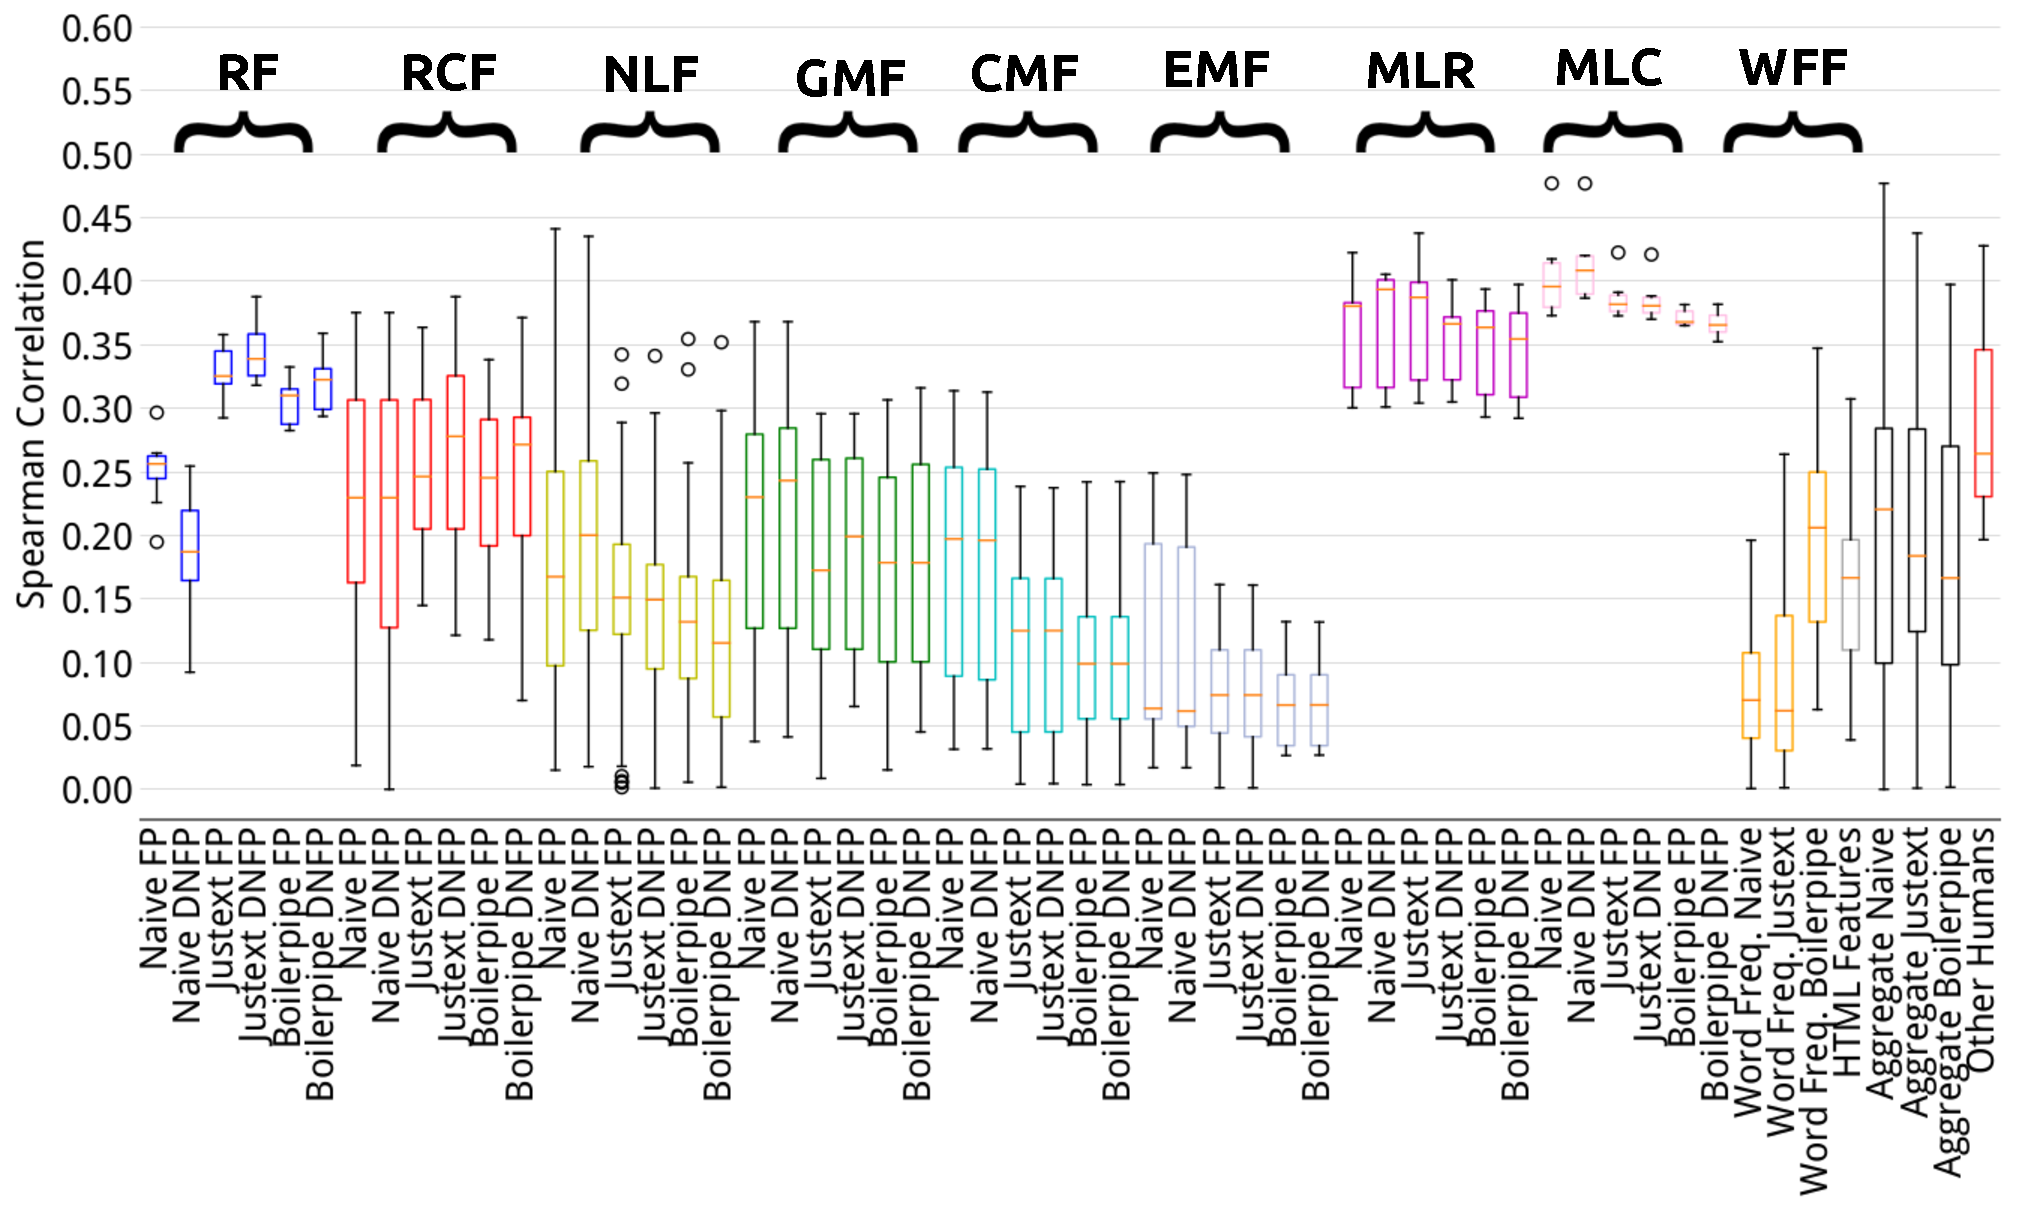
\includegraphics[width=0.85\textwidth]{graphics/box_spearman15_raw_values_joao}\vspace{-7pt}
	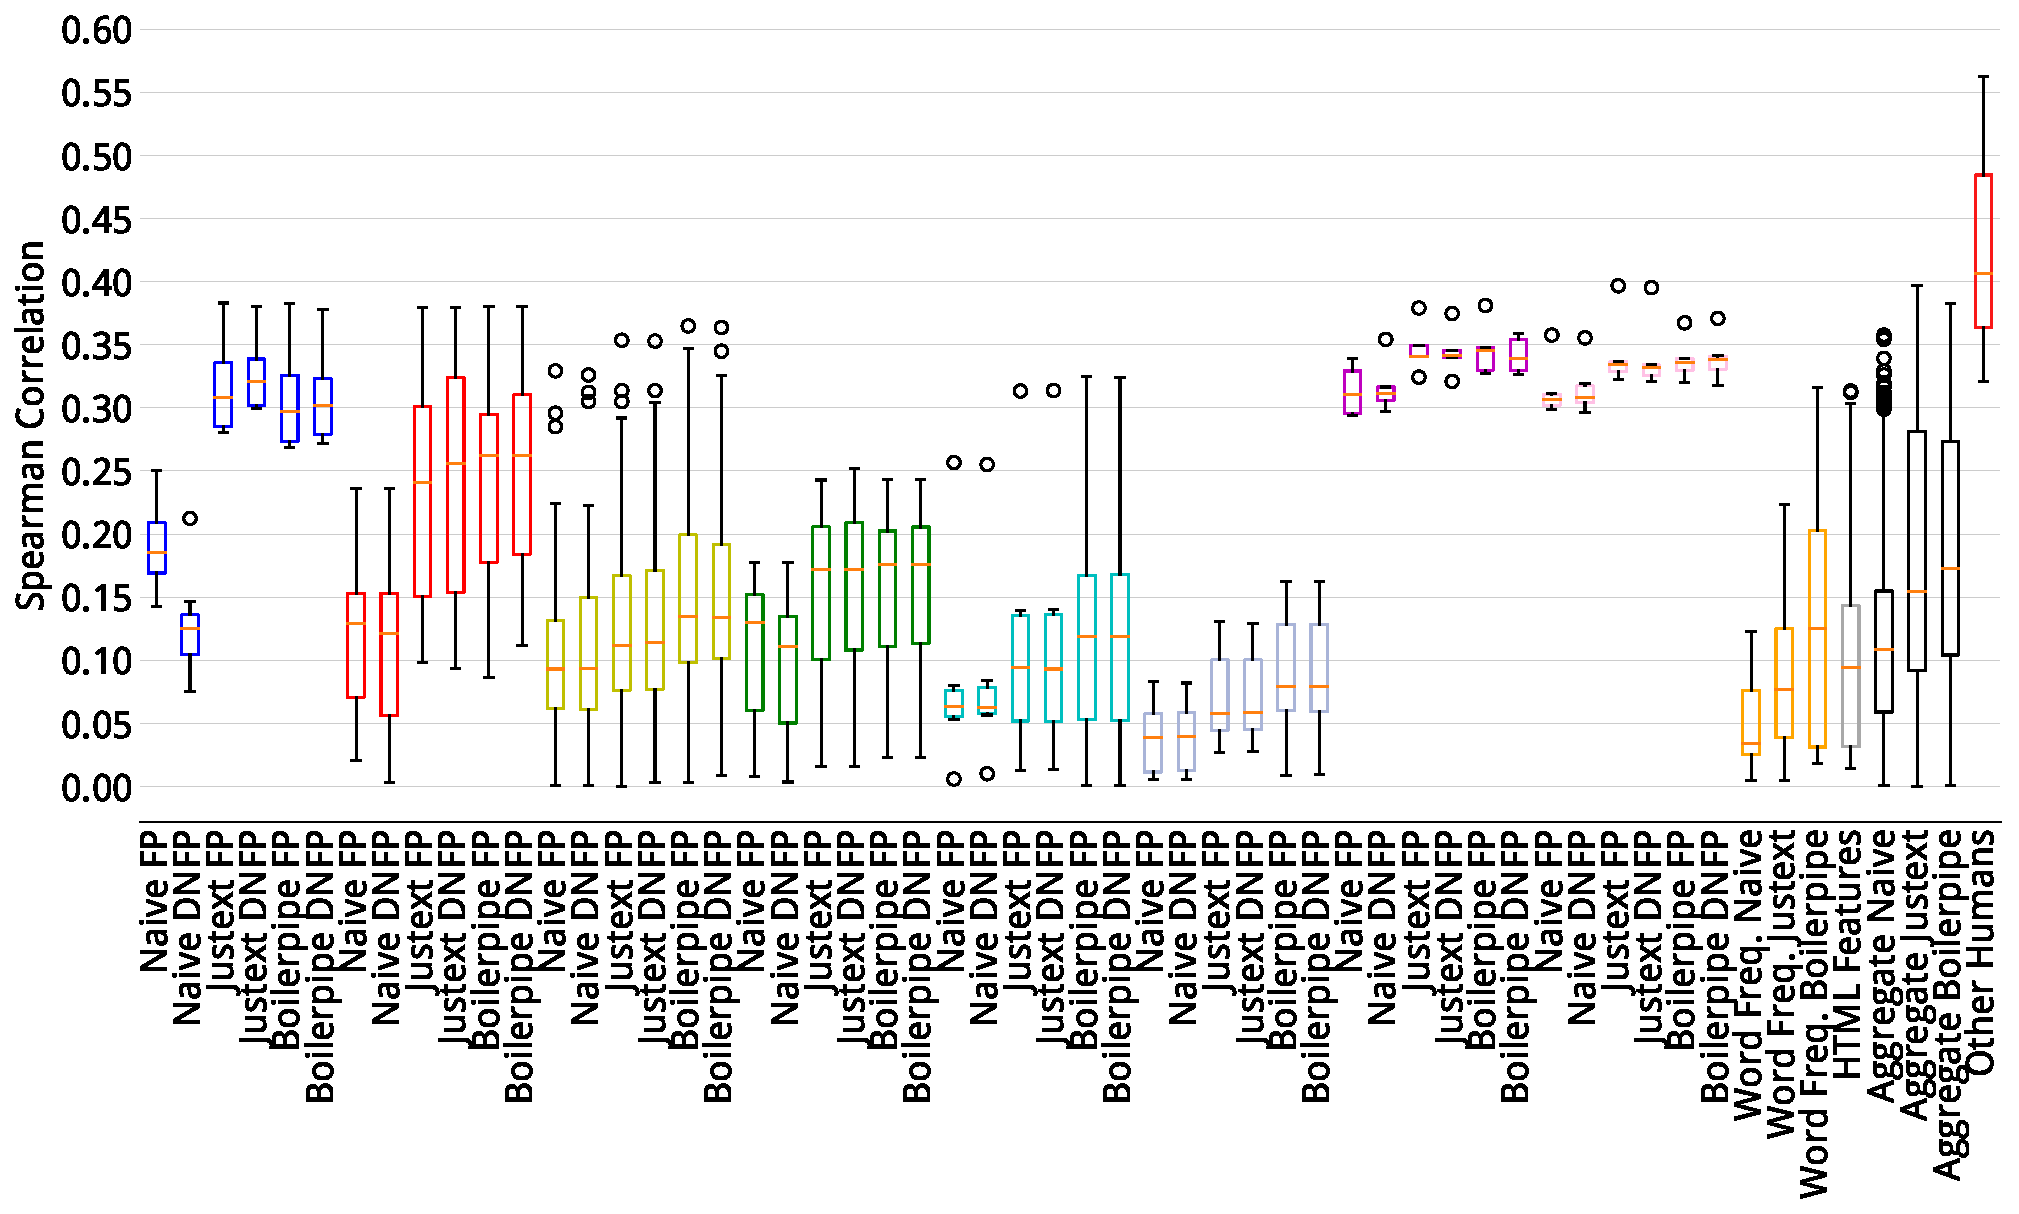
\includegraphics[width=0.85\textwidth]{graphics/box_spearman16_raw_values}
	\caption{Correlations between understandability estimators and human assessments for CLEF 2015 (top) and 2016 (bottom). For example, the first boxplot on the top represents the distribution of Spearman correlations with human assessments across all features in the category Readability Features (Table~\ref{tab:doc_features}), obtained with the Naive \textit{ForcePeriod} preprocessing, for CLEF 2015. Each box extends from the lower to the upper quartile values, with the red marker representing the median value for that category. Whiskers show the range of the data in each category and circles represent values considered outliers for the category (e.g., Spearman correlation for SMOG index was 0.296 and for ARI was 0.194: these were outliers for that category).} 
	\label{fig:boxplot_corr_docs}
	\vspace{-10pt}
\end{figure*}

We first examined the correlations between human assessments and readability formulae. We found that the \textit{Naive} preprocessing resulted in the lowest correlations, regardless of readability formula and heuristic (although \textit{DoNotForcePeriod} performed better than \textit{ForcePeriod}). Using Justext or Boilerplate resulted in higher correlations with human understandability assessments, and the \textit{ForcePeriod} heuristic was shown to be better than \textit{DoNotForcePeriod}. These results confirm the speculations of Palotti et al.~\cite{palotti15}: they found these settings to produce lower variances in understandability estimations and thus hypothesised that they were better suited to the task.

Overall, among readability formulae, the best results (highest correlations) were obtained by SMOG and DCI (see also Table~\ref{tab:top_corr_metrics}). Although no single setting outperformed the others in both collections, we found that the use of CLI and FRE with \textit{Justext} provided the most stable results across the collections, with correlations as high as the best ones in both collections.
These results confirmed the advice put forward by Palotti et al.~\cite{palotti15}, i.e. in general, if using readability measures, then CLI is to be preferred, along with an appropriate HTML extraction pipeline, regardless of the heuristic for sentence ending. We provide detailed plots to compare our results with Palotti's in the appendix.

When considering methods beyond those based on readability formulae, we found that the highest correlations were achieved by the regressors (MLR) and classifiers (MLC), independently of the preprocessing method used. There is little difference in terms of effectiveness of methods in these categories, with the exception of regressors on CLEF 2015 that exhibited not negligible variances: while for the Neural Network Regressor the Pearson correlation was 0.44, for the Support Vector Regressor it was only 0.30.

A common trend when comparing preprocessing pipelines is that the Naive pipeline provided the weakest correlations with human assessments for CLEF 2016, regardless of estimation methods and heuristics. This result, however, was not confirmed for CLEF 2015, where the Naive preprocessing negatively influenced correlations for the readability formula category (RF), but not for other categories, although it was generally associated with larger variances for the correlation coefficients.


\subsection*{Evaluation of Understandability Retrieval}
\label{sec:results}


\begin{table*}[ht!]
	\caption{Results obtained by integrating understandability estimations within
		retrieval methods on CLEF 2016. Baseline runs are reported at table
		indices 1-3 (the index column is labelled Idx). Re-ranking experiments
		are reported at indices 4-21. Fusion experiments are reported at indices
		22-30. Learning to rank experiments are reported at indices 31-35.
		All measures were calculated up to rank $n=10$. P-values are rounded to the third decimal digit and reported w.r.t GUIR run ($P_g$) and the BM25 baseline ($P_{bl}$). The highest result of each set of experiments is reported in bold face. }
	%; a p-value of 0.000 in the table means the p-value is $ \leq 0.000\overline{9}$
	%\vspace{-0.2cm}
	\label{tab:experiments} \resizebox{1.00\textwidth}{!}{ %
		\begin{tabular}{lcllll|clllclllclllcllllllllll}
			\toprule 
			\multirow{2}{*}{Idx}  & \multirow{2}{*}{\multirow{2}{*}{Rerank} } & \multirow{2}{*}{\multirow{2}{*}{Run} } & \multicolumn{8}{l}{Official CLEF 2016 Measures} & \multicolumn{18}{l}{New Measures to Evaluate Understandability in Retrieval }\tabularnewline
			\cmidrule(l{2pt}r{2pt}){4-10} \cmidrule(l{2pt}r{2pt}){11-29}  &  &  & $RBP$  & $P_{bl}$ & $P_{g}$ & Res.  & uRBP  & $P_{bl}$ & $P_{g}$ & Res.  & $RBP_{u}$  & $P_{bl}$ & $P_{g}$ & Res.  & $H_{rbp}$ & $P_{bl}$ & $P_{g}$ & Res.  & Unj  & $RBP_{r}^{*}$  & $P_{bl}$ & $P_{g}$ & $RBP_{u}^{*}$  & $P_{bl}$ & $P_{g}$ & $H_{rbp}^{*}$ & $P_{bl}$ & $P_{g}$\tabularnewline
			\midrule 
			1  & \multirow{3}{*}{No Rerank}  & GUIR~\cite{soldaini16} (Best Run)  & \textbf{28.11}  & - & - & 7.65  & \textbf{18.12}  & - & - & 7.19  & \textbf{45.69}  & - & - & 8.86  & \textbf{25.61}  & - & - & 6.50  & 0.01  & \textbf{28.29}  & - & - & \textbf{46.03}  & - & - & \textbf{25.79}  & - & -\tabularnewline
			2  &  & ECNU~\cite{song16} (2nd Best)  & 27.70  & - & .946 & 7.37  & 17.55  & - & .208 & \textbf{7.34}  & 43.89 & - & .012 & 8.66  & 25.35  & - & .763 & 6.26  & 0.01  & 27.77  & - & .635 & 44.18 & - & .009 & 25.48  & - & .660\tabularnewline
			3  &  & Plain BM25 Baseline  & 25.28 & - & .001 & \textbf{8.24}  & 16.05  & - & .000 & 6.94  & 42.08 & - & .000 & \textbf{10.97}  & 22.97 & - & .000 & \textbf{7.19}  & \textbf{0.06}  & 26.01  & - & .003 & 43.89  & - & .005 & 23.93  & - & .002\tabularnewline
			\midrule 
			4  & \multirow{3}{*}{\makecell{Dale-Chall \\Top 15}}  & Based on GUIR  & 24.29 & .000 & .000 & 8.89 & 16.62 & .001 & .001 & \textbf{7.27} & 48.96 & .000 & .000 & 11.05 & 24.76 & .193 & .193 & 7.61 & 0.03 & 24.83 & .000 & .000 & 50.56 & .000 & .000 & 25.38 & .521 & .521\tabularnewline
			5  &  & Based on ECNU  & 24.38 & .000 & .000 & 8.19 & 16.45 & .042 & .003 & 7.16 & 48.96 & .000 & .001 & 10.10 & 24.68 & .376 & .285 & 6.86 & 0.03 & 24.88 & .000 & .000 & 49.99 & .000 & .000 & 25.24 & .743 & .575\tabularnewline
			6  &  & Based on BM25  & 23.22 & .003 & .000 & 8.78 & 15.85 & .669 & .001 & 6.94 & 47.09 & .000 & .032 & 11.83 & 24.01 & .157 & .146 & 7.42 & 0.07 & 24.04 & .007 & .000 & 48.60 & .000 & .001 & 24.82 & .209 & .342\tabularnewline
			\hdashline 7  & \multirow{3}{*}{\makecell{Dale-Chall\\ Top 20}}  & Based on GUIR  & 21.86 & .000 & .000 & 10.04 & 15.15 & .000 & .000 & 7.05 & 48.54 & .004 & .004 & 13.13 & 22.94 & .000 & .000 & 8.68 & 0.06 & 23.23 & .000 & .000 & 51.78 & .000 & .000 & 24.44 & .048 & .048\tabularnewline
			8  &  & Based on ECNU  & 22.61 & .000 & .000 & 9.24 & 15.41 & .001 & .000 & 6.94 & 48.45 & .000 & .007 & 12.31 & 23.43 & .022 & .012 & 8.06 & 0.05 & 23.62 & .000 & .000 & 50.86 & .000 & .000 & 24.58 & .264 & .177\tabularnewline
			9  &  & Based on BM25  & 21.58 & .000 & .000 & 9.51 & 14.83 & .020 & .000 & 7.02 & 46.99 & .000 & .108 & 13.00 & 22.89 & .849 & .009 & 8.06 & 0.09 & 22.93 & .000 & .000 & 49.55 & .000 & .000 & 24.26 & .769 & .125\tabularnewline
			\hdashline 10  & \multirow{3}{*}{\makecell{Dale-Chall\\ Top 50}}  & Based on GUIR  & 16.07 & .000 & .000 & 15.31 & 11.50 & .000 & .000 & 6.80 & 41.41 & .001 & .001 & 24.34 & 17.95 & .000 & .000 & 14.48 & 0.23 & 20.80 & .000 & .000 & 53.07 & .000 & .000 & 23.14 & .011 & .011\tabularnewline
			11  &  & Based on ECNU  & 16.72 & .000 & .000 & 17.64 & 11.67 & .000 & .000 & \textbf{7.27} & 40.46 & .005 & .000 & 24.18 & 18.13 & .000 & .000 & \textbf{15.87} & 0.24 & 21.38 & .000 & .000 & 52.10 & .000 & .000 & 23.41 & .036 & .023\tabularnewline
			12  &  & Based on BM25  & 15.06 & .000 & .000 & 15.35 & 10.55 & .000 & .000 & 6.62 & 40.03 & .156 & .000 & 23.88 & 16.55 & .000 & .000 & 13.83 & 0.24 & 19.42 & .000 & .000 & 51.69 & .000 & .000 & 21.59 & .012 & .000\tabularnewline
			\hdashline 13  & \multirow{3}{*}{\makecell{XGB\\ Top 15}}  & Based on GUIR  & \textbf{25.16} & .000 & .000 & 8.09 & \textbf{17.27} & .047 & .047 & 7.12 & \textbf{50.96} & .000 & .000 & 10.11 & \textbf{25.16} & .456 & .456 & 6.89 & 0.02 & \textbf{25.61} & .000 & .000 & 52.00 & .000 & .000 & \textbf{25.68} & .853 & .853\tabularnewline
			14  &  & Based on ECNU  & 24.18 & .000 & .000 & 7.69 & 16.54 & .086 & .009 & 7.09 & 50.00 & .000 & .000 & 9.91 & 24.56 & 0.224 & .181 & 6.65 & 0.02 & 24.56 & .000 & .000 & 50.74 & .000 & .000 & 25.01 & .435 & .326\tabularnewline
			15  &  & Based on BM25  & 22.79 & .002 & .000 & 7.94 & 15.64 & .585 & .000 & 6.84 & 47.88 & .000 & .006 & 11.65 & 23.10 & 0.835 & .009 & 7.08 & 0.07 & 23.46 & .001 & .000 & 49.12 & .000 & .000 & 23.80 & .912 & .025\tabularnewline
			\hdashline 16  & \multirow{3}{*}{\makecell{XGB\\ Top 20}}  & Based on GUIR  & 22.38 & .000 & .000 & 9.49 & 15.61 & .000 & .000 & 7.05 & 50.45 & .000 & .000 & 12.08 & 23.30 & .001 & .001 & 8.16 & 0.05 & 23.62 & .000 & .000 & 52.98 & .000 & .000 & 24.68 & .068 & .068\tabularnewline
			17  &  & Based on ECNU  & 22.95 & .000 & .000 & 8.82 & 15.95 & .010 & .001 & 7.02 & 50.42 & .000 & .000 & 11.70 & 23.97 & .081 & .046 & 7.56 & 0.04 & 23.68 & .000 & .000 & 52.15 & .000 & .000 & 24.73 & .317 & .202\tabularnewline
			18  &  & Based on BM25  & 20.77 & .000 & .000 & 9.26 & 14.51 & .009 & .000 & 6.76 & 47.85 & .000 & .019 & 13.24 & 22.04 & .215 & .000 & 8.24 & 0.08 & 22.10 & .000 & .000 & 50.28 & .000 & .000 & 23.32 & .410 & .010\tabularnewline
			\hdashline 19  & \multirow{3}{*}{\makecell{XGB\\ Top 50}}  & Based on GUIR  & 16.65 & .000 & .000 & 15.73 & 12.39 & .000 & .000 & 6.84 & 43.49 & .042 & .042 & 23.63 & 18.70 & .000 & .000 & 13.74 & 0.22 & 21.13 & .000 & .000 & \textbf{55.07} & .000 & .000 & 23.58 & .016 & .016\tabularnewline
			20  &  & Based on ECNU  & 16.19 & .000 & .000 & 17.01 & 11.82 & .000 & .000 & \textbf{7.27} & 43.05 & .184 & .009 & \textbf{24.75} & 18.27 & .000 & .000 & 14.41 & 0.24 & 20.16 & .000 & .000 & 54.70 & .000 & .000 & 22.96 & .006 & .003\tabularnewline
			21  &  & Based on BM25  & 15.55 & .000 & .000 & 14.92 & 11.44 & .000 & .000 & 6.59 & 42.29 & .791 & .026 & 23.21 & 17.60 & .000 & .000 & 13.00 & \textbf{0.25} & 19.58 & .000 & .000 & 53.94 & .000 & .000 & 22.19 & .043 & .000\tabularnewline
			\midrule 
			22  & \multirow{3}{*}{\makecell{RRF (XGB \& Orig.)\\ Top 15} }  & Based on GUIR  & 27.23 & .027 & .027 & 7.76 & 18.31 & .560 & .560 & 7.23 & 49.69 & .000 & .000 & 9.18 & 26.46 & .021 & .021 & 6.62 & 0.01 & 27.46 & .035 & .035 & 50.07 & .000 & .000 & 26.69 & .013 & .013\tabularnewline
			23  &  & Based on ECNU  & 26.60 & .014 & .030 & 7.41 & 17.81 & .277 & .646 & 7.19 & 48.67 & .000 & .000 & 8.80 & 26.02 & .099 & .327 & 6.09 & 0.01 & 26.76 & .024 & .021 & 49.10 & .000 & .000 & 26.27 & .050 & .286\tabularnewline
			24  &  & Based on BM25  & 24.64 & .160 & .000 & 8.13 & 16.50 & .109 & .004 & 6.98 & 46.57 & .000 & .103 & 11.02 & 24.14 & .004 & .080 & 7.11 & 0.06 & 25.39 & .151 & .000 & 48.25 & .000 & .002 & 25.04 & .004 & .434\tabularnewline
			\hdashline 25  & \multirow{3}{*}{\makecell{RRF (XGB \& Orig.)\\ Top 20}}  & Based on GUIR  & 26.21 & .000 & .000 & 7.96 & 17.73 & .169 & .169 & 7.19 & 50.29 & .000 & .000 & 9.58 & 25.89 & .536 & .536 & 6.73 & 0.03 & 26.53 & .000 & .000 & 50.98 & .000 & .000 & 26.25 & .280 & .280\tabularnewline
			26  &  & Based on ECNU  & 26.15 & .002 & .004 & 7.64 & 17.69 & .561 & .412 & 7.09 & 49.70 & .000 & .000 & 9.28 & 26.07 & .140 & .345 & 6.39 & 0.02 & 26.38 & .010 & .004 & 50.32 & .000 & .000 & 26.35 & .067 & .265\tabularnewline
			27  &  & Based on BM25  & 24.10 & .029 & .000 & 8.26 & 16.34 & .328 & .003 & 6.91 & 47.62 & .000 & .009 & 11.34 & 24.10 & .017 & .089 & 7.37 & 0.06 & 24.92 & 0.031 & .000 & 49.37 & .000 & .000 & 25.03 & .017 & .452\tabularnewline
			\hdashline 28  & \multirow{3}{*}{\makecell{RRF (XGB \& Orig.)\\ Top 50}}  & Based on GUIR  & 24.09 & .000 & .000 & 9.44 & 16.85 & .003 & .003 & 7.02 & 50.55 & .000 & .000 & 11.76 & 24.76 & .122 & .122 & 8.01 & 0.07 & 25.08 & .000 & .000 & 52.84 & .000 & .000 & 25.84 & .974 & .974\tabularnewline
			29  &  & Based on ECNU  & 24.17 & .000 & .000 & 8.67 & 16.75 & .160 & .021 & 7.12 & 50.63 & .000 & .000 & 11.66 & 25.00 & .614 & .453 & 7.61 & 0.07 & 24.90 & .000 & .000 & 52.50 & .000 & .000 & 25.84 & .624 & .991\tabularnewline
			30  &  & Based on BM25  & 22.32 & .000 & .000 & 8.82 & 15.51 & .425 & .000 & 6.73 & 48.78 & .000 & .001 & 12.84 & 23.14 & .787 & .008 & 7.78 & 0.10 & 23.45 & .001 & .000 & 51.85 & .000 & .000 & 24.53 & .358 & .127\tabularnewline
			\midrule 
			31  & \multirow{5}{*}{XGB LeToR}  & LTR 1 on BM25  & 20.42 & .000 & .000 & 17.61 & 13.00 & .000 & .000 & 7.41 & 32.17 & .000 & .000 & 24.61 & 18.39 & .000 & .000 & 14.41 & 0.28 & 25.25 & .200 & .003 & 43.19 & .214 & .001 & 23.83 & .685 & .038\tabularnewline
			32  &  & LTR 2 on BM25  & 25.16 & .129 & .000 & 19.95 & 15.85 & .096 & .000 & 8.09 & 34.31 & .000 & .000 & 24.95 & 21.69 & .109 & .000 & 17.43 & 0.28 & 30.60 & .008 & .370 & 45.37 & .378 & .147 & 27.57 & .001 & .062\tabularnewline
			33  &  & LTR 3 on BM25  & 26.35 & .115 & .005 & \textbf{20.48} & 15.88 & .023 & .000 & 8.16 & 34.73 & .000 & .000 & 24.69 & 21.81 & .075 & .000 & 17.41 & 0.22 & 32.25 & .006 & .126 & 45.44 & .728 & .059 & 28.22 & .000 & .021\tabularnewline
			34  &  & LTR 4 on BM25  & 16.16 & .000 & .000 & 19.48 & 10.76 & .000 & .000 & 7.27 & \textbf{36.75} & .000 & .000 & \textbf{28.51} & 16.77 & .000 & .000 & \textbf{17.80} & \textbf{0.29} & 22.20 & .000 & .000 & \textbf{50.06} & .000 & .042 & 23.32 & .343 & .031\tabularnewline
			35  &  & LTR 5 on BM25  & \textbf{26.76} & .196 & .002 & \textbf{20.48} & \textbf{16.19} & .067 & .000 & \textbf{8.34} & 35.26 & .000 & .000 & 24.13 & \textbf{22.96} & .559 & .008 & 17.59 & 0.22 & \textbf{32.60} & .003 & .120 & 45.87 & .375 & .228 & \textbf{29.20} & .000 & .001\tabularnewline
			\bottomrule
	\end{tabular}} % end of resizebox
\end{table*}



Results for the considered retrieval methods are reported in Table~\ref{tab:experiments}. We report only the results for CLEF 2016 for brevity; those for CLEF 2015 exhibited similar trends and are included in the appendix. 
As both the RBP residuals and the column \textit{Unj} quantify the effect unassessed documents have on evaluation, we opt to show the RBP residuals only in the supplementary appendix and show \textit{Unj} here, as its interpretation is straightforward: \textit{Unj} is the average percentage of documents without assessment in the top 10 results. Larger values of \textit{Unj} entail that actual effectiveness may be sensibly larger. Here we also show the values for the condensed measures. 

In Table~\ref{tab:experiments}, statistical significance was measured with respect to the best CLEF 2016 run, GUIR (p-values indicated with $P_g$), and the BM25 baseline (p-values indicated with $P_{bl}$). A two-tailed paired t-test was used to compute statistical significance; note that the baseline BM25 is significantly worse than GUIR across all measures.

The effectiveness of the top two submissions to CLEF 2016 and the BM25 baseline are reported at indices 1-3 of Table~\ref{tab:experiments}. 
In turn, we report the results of each sub-experiment: \textit{Simple re-ranking} (indices 4-21), \textit{Fusion Experiments} (indices 22-30), \textit{Learning to rank} (indices 31-35).

\textbf{\textit{Simple Re-ranking:}} Indices 4-12 of Table~\ref{tab:experiments} report the results of re-ranking methods applied to the runs listed at indices 1-3. Re-ranking was applied based on the DCI score of each document calculated using the preprocessing combination of Boilerpipe and ForcePeriod (best according to Pearson correlation, from Table~\ref{tab:top_corr_metrics}).
We found that the relevance of the re-ranked runs (as measured by $RBP_r$ and $RBP_r^*$) significantly decreased, compared to the original runs: e.g., re-ranking the top 15 search results using DCI  made $RBP_r$ decrease from 25.28 to 21.58. However, as expected, these re-ranked results were significantly more understandable: for the previous example, $RBP_u$ passed from 42.08 to 47.09.

In the experiments, we also studied the influence of the number of documents considered for re-ranking (cut-off). Indices 4-6 refer to re-ranking only the top $k=15$ documents from the original runs; 7-9 refer to the first $k=20$; and 10-12 to the first $k=50$. The results show that the more documents are considered for re-ranking, the more degradation in $RBP_r$ effectiveness. Considering understandability-only in the evaluation shows mixed results. Similar trends were observed for evaluation measures that consider understandability ($RBP$ and $RBP_u$), however with some exceptions. For example, an increase in $uRBP$ was observed when re-ranking ECNU using the top 50 results. 

Note that with the increase of the number of documents considered for re-ranking, there is an increase in the number of unassessed documents being considered by the evaluation measures. 
Nevertheless, we note that if unassessed documents are excluded from the evaluation, similar trends are observed, e.g., compare findings with those for the condensed measures $uRBP^*$, $RBP_r^*$, $RBP_u^*$ and $H_{RBP}^*$.

Indices 13-21 refer to using the XGB regressor trained with all features listed in Table~\ref{tab:doc_features} to estimate understandability. Similarly to when using DCI, as the cut-off increased, e.g., from $k=15$ to $k=50$, the documents returned were more understandable but less relevant. For the same cut-off value, e.g., $k=15$, the machine learning method used for estimating understandability consistently yielded more understandable results than DCI (higher $RBP_u$ and $RBP_u^*$). 

Overall, statistically significant improvements over the baselines were observed for most configurations and measures.  

\textit{\textbf{Rank Fusion:}} Next, we report the results of automatically combining topical relevance and understandability through rank fusion (indices 22 to 30). We used the XGB method for estimating understandability, as it was the one yielding highest effectiveness for the re-ranking method. Runs were thus produced by fusing the re-ranking with XGB and the original run. (Results for DCI are reported in the appendix and confirm the superiority of XGB.) 

As for re-ranking, also for the rank fusion approaches we found that, in general, higher cut-offs were associated to higher effectiveness in terms of understandability measures on one hand, but higher losses in terms of relevance-oriented measures on the other. Overall, results obtained with rank fusion were superior to those obtained with re-ranking only, though most differences were not statistically significant. Statistically significant improvements over the baselines were instead observed for most configurations and measures.  

\textit{\textbf{Learning to Rank:}} Last, we analyse the results obtained by the learning to rank methods (indices 31-35). Unlike with the previous methods, we did not impose a rank cut-off on learning to rank. Learning to rank was only applied to the BM25 baseline, as we had no access to the IR features for the runs submitted at CLEF (i.e. GUIR and ECNU for CLEF 2016).

When considering $RBP_r$ and $uRBP$, learning to rank exhibited effectiveness that was significantly inferior to that of the GUIR and ECNU baseline runs, though higher than those for the BM25 baseline (for some configurations). The examination of the number of unassessed documents (and the RBP residuals, see appendix) revealed that this may have been because measures were affected by the large number of unassessed documents retrieved in the top 10 ranks. For example, the $RBP_r$ residual for learning to rank methods was about double that of the baselines or other approaches (see appendix). In fact, among the documents retrieved in the top 10 results by learning to rank, there were 20\% that were unassessed, compared to an average of 3\% for the other methods. (Excluding XGB with cut-off 50, which also exhibited high residuals). 

We thus should carefully account for unassessed documents through considering the residuals of RBP measures, as well as the condensed measures. When this was done, we observed that learning to rank methods overall provided substantial gains over the original runs and other methods (when considering $RBP^*_r$, $RBP^*_u$ and $H_{RBP}^*$), or large potential gains over these methods (when considering the residuals). Next, we analyse these results in more detail. 

No improvements over the baselines were found for LTR 1 (index 31), and the high residuals for $RBP_r$ were not matched by other residuals or by considering only assessed documents (see appendix). LTR 1 was a simple method that used only IR features and was trained only on topical relevance. Specifically, we devised 24 IR features using the Terrier framework. The score of various retrieval models was extracted from a multi-field index composed of title, body and whole document. Although simple, this is a typical learning to rank setting.

Compared to LTR 1, LTR 2 (index 32) included the understandability features listed in Table~\ref{tab:doc_features}. This inclusion was as beneficial to the understandability measures as to the relevance measures, with $RBP_r^*$, $RBP_u^*$ and $H_{RBP}^*$ all showing gains over the baselines. LTR 3 obtained similar $H_{RBP}^*$ values, though with higher effectiveness for relevance measures ($RBP_r^*$) than for understandability ($RBP_u^*$).

LTRs 4 and 5 were devised based on a set understandability threshold $U=40$. While LTR 4 took into consideration only documents that were easy-to-read (understandability label $\le$ $U$), LTR 5 considered all documents, but boosted the relevance score. LTR 4 reached the highest understandability score for the learning-to-rank approaches ($RBP_u^{*}=50.06$), but it failed to retrieve a substantial number of relevant documents ($RBP_r^{*}=22.20$). In turn, LTR 5 reached the highest
understandability-relevance trade-off ($H_{RBP}^{*}=29.20$). Compared to the BM25 baseline (on which it was based), LTR 5  largely increased both relevance ($RBP_r^*$ from 26.01 to 32.60 -- a 25\% increase, $P_{bl}=0.003$) and understandability ($RBP_u^*$ from 43.89 to 45.87 -- a 4\% increase, $P_{bl}<0.001$). Note that LTR 5 was also significantly better than the best run submitted to CLEF 2016 for both $RBP_r^{*}$ (15\% increase, $P_{g}=0.120$) and $H_{RBP}^{*}$ (13\% increase, $P_{g}=0.001$).


\section*{Discussion}

\subsection*{Principal Findings}

The empirical experiments suggested that:

\vspace{-4pt}
\begin{enumerate}[leftmargin=*]
	\item Machine learning methods based on regression are best suited to estimate the understandability of health Web pages;
	\item Preprocessing does affect effectiveness (both for understandability prediction and document retrieval), although, compared to other methods, ML-based methods for understandability estimation are less subject to variability caused by poor preprocessing;
	\item Learning to rank methods can be specifically trained to promote more understandable search results, while still providing an effective trade-off with topical relevance.
\end{enumerate} 


\subsection*{Limitations}
In this work, we relied on data collected through the CLEF 2015 and CLEF 2016 evaluation efforts to evaluate the effectiveness of methods that estimate the understandability of the Web pages. These assessments were obtained by asking medical experts and practitioners to rate documents;  although they were asked to estimate the understandability of the content as if they were the patients they treat, there may have been noise and imprecisions in the collection mechanism due to the subjectivity of the
task. Figure~\ref{fig:boxplot_corr_docs} highlights this by showing that the agreement between assessors is relatively low. A better setting may have been to directly recruit health consumers: the task would still have been subjective, but would have captured real ratings, rather than inferred or perceived ratings. Despite this, our previous work has shown that no substantial differences were found in the downstream evaluation of retrieval systems, when we acquired understandability assessments from health consumers for a subset of the CLEF 2015 collection~\cite{palotti16b}. 

Relevance assessments on the CLEF 2015 and 2016 collections are incomplete~\cite{clef15,clef16}, i.e. not all top ranked web pages retrieved by the investigated methods have an explicit relevance assessment. This is often the case in information retrieval, where the validity of experiments based on incomplete assessments has been thoroughly investigated~\cite{sanderson2010test}. Nonetheless, we carefully controlled for the impact unassessed documents had in our experiments by measuring their number and using measures like RBP that account for residuals and condensed variants. The residuals analysis has been reported in the appendix. 

The methods investigated here do not provide a fully personalised search, with respect to how much of the health content consumers with different health knowledge may be able to understand. Instead, we focus on making the results understandable by anyone: and thus promote in the search results content that has the highest level of understandability. However, people with a more than average medical knowledge may benefit higher from more specialised content. We leave this personalisation aspect, i.e., the tailoring of the understandability level of the promoted content with respect to the user's knowledge and abilities, to further work.

\subsection*{Conclusions}

We have examined approaches to estimate the understandability of health Web pages, including the impact of HTML preprocessing techniques, and how to integrate these within retrieval methods to provide more understandable search results for people seeking health information. We found that machine learning methods are better suited than traditionally employed readability measures for assessing the understandability of health related web pages and that learning to rank is the most effective strategy to integrate this into retrieval. We also found that HTML and text pre-processing do affect the effectiveness of both understandability estimations and of the retrieval process, although machine learning methods are less sensitive to this issue.

This article contributes to improving search engines tailored to consumer health search because it thoroughly investigates promises and pitfalls of understandability estimations and their integration into retrieval methods. The article further highlights which methods and settings should be used to provide better search results to health information seekers. As shown in Figure~\ref{fig:dist}, these methods would clearly improve current health-focused search engines. 

The methods investigated here do not provide a fully personalised search, with respect to how much of the health content consumers with different health knowledge may be able to understand. Instead, we focus on making the results understandable by anyone: and thus promote in the search results content that has the highest level of understandability. However, people with a more than average medical knowledge may benefit higher from more specialised content. We leave this personalisation aspect, i.e., the tailoring of the understandability level of the promoted content with respect to the user's knowledge and abilities, to further work.

\subsection*{Acknowledgment}
The authors acknowledge the TU Wien University Library for financial support through its Open Access Funding Programme.


\begin{thebibliography}{10}

    \bibitem{zhang2014multidimensional}
	Zhang Y, Zhang J, Lease M, Gwizdka J.
	\newblock Multidimensional relevance modeling via psychometrics and
	crowdsourcing.
	\newblock In: Proceedings of the 37th international ACM SIGIR conference on
	Research \& development in information retrieval. ACM; 2014. p. 435--444.
	\newblock \href {http://dx.doi.org/10.1145/2600428.2609577}
	{doi:10.1145/2600428.2609577}.
	
	\bibitem{white09b}
	White RW, Horvitz E.
	\newblock Cyberchondria: Studies of the Escalation of Medical Concerns in Web
	Search.
	\newblock ACM Transactions on Information Systems. 2009 Nov;27(4):23:1--23:37.
	\newblock \href {http://dx.doi.org/10.1145/1629096.1629101}
	{doi:10.1145/1629096.1629101}.
	
	\bibitem{white13}
	White R.
	\newblock Beliefs and biases in web search.
	\newblock In: Proceedings of the 36th international ACM SIGIR conference on
	Research and development in information retrieval. SIGIR '13. New York, NY,
	USA: ACM; 2013. p. 3--12.
	\newblock \href {http://dx.doi.org/10.1145/2484028.2484053}
	{doi:10.1145/2484028.2484053}.
	
	\bibitem{graber99}
	Graber MA, Roller CM, Kaeble B.
	\newblock Readability levels of patient education material on the World Wide
	Web.
	\newblock Journal of Family Practice. 1999;48(1):58--59.
	\newblock Available from: \url{https://www.ncbi.nlm.nih.gov/pubmed/9934385}.
	
	\bibitem{fitzsimmons10}
	Fitzsimmons P, Michael B, Hulley J, Scott G.
	\newblock A readability assessment of online Parkinson's disease information.
	\newblock The journal of the Royal College of Physicians of Edinburgh.
	2010;40(4):292--296.
	\newblock Available from: \url{https://www.ncbi.nlm.nih.gov/pubmed/21132132}.
	
	\bibitem{wiener13}
	Wiener RC, Wiener-Pla R.
	\newblock Literacy, pregnancy and potential oral health changes: The internet
	and readability levels.
	\newblock Maternal and child health journal. 2014;18(3):657--662.
	\newblock Available from: \url{https://www.ncbi.nlm.nih.gov/pubmed/23784613}.
	
	\bibitem{patel13}
	Patel CR, Cherla DV, Sanghvi S, Baredes S, Eloy JA.
	\newblock Readability assessment of online thyroid surgery patient education
	materials.
	\newblock Head \& neck. 2013;35(10):1421--1425.
	\newblock Available from: \url{https://www.ncbi.nlm.nih.gov/pubmed/22972634}.
	
	\bibitem{meillier17}
	Meillier A, Patel S.
	\newblock Readability of Healthcare Literature for Gastroparesis and Evaluation
	of Medical Terminology in Reading Difficulty.
	\newblock Gastroenterology Research. 2017;10(1):1--5.
	\newblock Available from: \url{https://www.ncbi.nlm.nih.gov/pubmed/28270870}.
	
	\bibitem{ellimoottil12}
	Ellimoottil C, Polcari A, Kadlec A, Gupta G.
	\newblock Readability of websites containing information about prostate cancer
	treatment options.
	\newblock The Journal of urology. 2012;188(6):2171--2176.
	\newblock Available from: \url{https://www.ncbi.nlm.nih.gov/pubmed/23083852}.
	
   	\bibitem{gabrilovich2016cura}
	Gabrilovich E.
	\newblock Cura Te Ipsum: answering symptom queries with question intent.
	\newblock In: Second WebQA workshop, SIGIR 2016 (invited talk); 2016.
	WebCitation: \url{http://www.webcitation.org/6yHTeM33k}.
	\newblock Available from:
	\url{http://plg2.cs.uwaterloo.ca/~avtyurin/WebQA2016/}.
	
    \bibitem{boyer15}
    Boyer, C, Dolamic, L.
    \newblock Automated detection of HONcode website conformity compared to manual 
    detection: an evaluation.
    \newblock In: Journal of medical Internet research. 2015; 17:6.
    \newblock \href {http://doi.org/10.2196/jmir.3831}
    {10.2196/jmir.3831}.

	\bibitem{clef16}
	Zuccon G, Palotti J, Goeuriot L, Kelly L, Lupu M, Pecina P, et~al.
	\newblock {The IR Task at the CLEF eHealth evaluation lab 2016: user-centred
		health information retrieval}.
	\newblock In: {CLEF 2016-Conference and Labs of the Evaluation Forum}. vol.
	1609; 2016. p. 15--27.
	\newblock Available from: \url{http://ceur-ws.org/Vol-1609/16090015.pdf}.

	\bibitem{palotti15}
	Palotti J, Zuccon G, Hanbury A.
	\newblock The Influence of Pre-processing on the Estimation of Readability of
	Web Documents.
	\newblock In: Proceedings of the 24th ACM International on Conference on
	Information and Knowledge Management. CIKM '15. New York, NY, USA: ACM; 2015.
	p. 1763--1766.
	\newblock \href {http://dx.doi.org/10.1145/2806416.2806613}
	{doi:10.1145/2806416.2806613}.
	
	\bibitem{palotti2016ranking}
	Palotti J, Goeuriot L, Zuccon G, Hanbury A.
	\newblock Ranking health web pages with relevance and understandability.
	\newblock In: Proceedings of the 39th international ACM SIGIR conference on
	Research and development in information retrieval. ACM; 2016. p. 965--968.
	\newblock Available from: \url{10.1145/2911451.2914741}.
	
	\bibitem{cowan04}
	Cowan CF.
	\newblock Teaching patients with low literacy skills.
	\newblock Jones \& Bartlett Learning; 2004.
	\newblock ISBN 978-0397551613.
	
	\bibitem{wallace04}
	Wallace LS, Lennon ES.
	\newblock American Academy of Family Physicians patient education materials:
	can patients read them?
	\newblock Family medicine. 2004;36(8):571--574.
	\newblock Available from: \url{https://www.ncbi.nlm.nih.gov/pubmed/15343418}.
	
	\bibitem{davis04}
	Davis TC, Wolf MS.
	\newblock Health literacy: implications for family medicine.
	\newblock Family Medicine. 2004;36(8):595--598.
	\newblock Available from: \url{https://www.ncbi.nlm.nih.gov/pubmed/15343422}.
	
	\bibitem{stossel12}
	Stossel LM, Segar N, Gliatto P, Fallar R, Karani R.
	\newblock Readability of patient education materials available at the point of
	care.
	\newblock Journal of general internal medicine. 2012;27(9):1165--1170.
	\newblock Available from: \url{https://www.ncbi.nlm.nih.gov/pubmed/22528620}.
	
	\bibitem{clear94}
	{National Cancer Institute}.
	\newblock {Clear \& Simple: Developing Effective Print Materials for
		Low-literate Readers}.
	\newblock NIH publication. National Institutes of Health; Accessed: 2017-09.
	WebCitation: \url{http://www.webcitation.org/6yHTsSTK7}.
	\newblock Available from:
	\url{https://www.nih.gov/institutes-nih/nih-office-director/office-communications-public-liaison/clear-communication/clear-simple}.
	
	\bibitem{shoemaker2014development}
	Shoemaker SJ, Wolf MS, Brach C.
	\newblock Development of the Patient Education Materials Assessment Tool
	(PEMAT): a new measure of understandability and actionability for print and
	audiovisual patient information.
	\newblock Patient education and counseling. 2014;96(3):395--403.
	\newblock Available from: \url{https://www.ncbi.nlm.nih.gov/pubmed/24973195}.
	
	\bibitem{becker04}
	Becker SA.
	\newblock A study of web usability for older adults seeking online health
	resources.
	\newblock ACM Transactions on Computer-Human Interaction (TOCHI).
	2004;11(4):387--406.
	\newblock \href {http://dx.doi.org/10.1145/1035575.1035578}
	{doi:10.1145/1035575.1035578}.
	
	\bibitem{zheng2017readability}
	Zheng J, Yu H.
	\newblock Readability formulas and user perceptions of electronic health
	records difficulty: a corpus study.
	\newblock Journal of medical Internet research. 2017;19(3).
	\newblock \href {http://dx.doi.org/10.2196/jmir.6962} {doi:10.2196/jmir.6962}.
	
	\bibitem{cli75}
	Coleman M, Liau TL.
	\newblock {A Computer Readability Formula Designed for Machine Scoring}.
	\newblock Journal of Applied Psychology. 1975;\href
	{http://dx.doi.org/10.1037/h0076540} {doi:10.1037/h0076540}.
	
	\bibitem{dale48}
	Dale E, Chall JS.
	\newblock A Formula for Predicting Readability: Instructions.
	\newblock Educational Research Bulletin. 1948;27(2):37--54.
	\newblock Available from: \url{http://www.jstor.org/stable/1473669}.
	
	\bibitem{flesch75}
	Kincaid J, Fishburne R, Rogers R, Chissom B.
	\newblock {Derivation of New Readability Formulas for Navy Enlisted Personnel}.
	\newblock National Technical Information Service; 1975.
	\newblock Available from:
	\url{http://www.dtic.mil/dtic/tr/fulltext/u2/a006655.pdf}.
	
	\bibitem{dubay04}
	Dubay WH.
	\newblock The Principles of Readability.
	\newblock Costa Mesa, CA: Impact Information. 2004;\href
	{http://dx.doi.org/10.1.1.91.4042} {doi:10.1.1.91.4042}.
	
	\bibitem{liu04}
	Liu X, Croft WB, Oh P, Hart D.
	\newblock Automatic Recognition of Reading Levels from User Queries.
	\newblock In: Proceedings of the 27th Annual International ACM SIGIR Conference
	on Research and Development in Information Retrieval. SIGIR '04. ACM; 2004.
	p. 548--549.
	\newblock \href {http://dx.doi.org/10.1145/1008992.1009114}
	{doi:10.1145/1008992.1009114}.
	
	\bibitem{collins05}
	Collins-Thompson K, Callan J.
	\newblock Predicting reading difficulty with statistical language models.
	\newblock Journal of the Association for Information Science and Technology.
	2005;56(13):1448--1462.
	\newblock \href {http://dx.doi.org/10.1002/asi.20243} {doi:10.1002/asi.20243}.
	
	\bibitem{heilman07}
	Heilman M, Collins-Thompson K, Callan J, Eskenazi M.
	\newblock Combining lexical and grammatical features to improve readability
	measures for first and second language texts.
	\newblock In: Human Language Technologies 2007: The Conference of the North
	American Chapter of the Association for Computational Linguistics;
	Proceedings of the Main Conference; 2007. p. 460--467.
	\newblock Available from: \url{10.1.1.70.1391}.
	
	\bibitem{pitler08}
	Pitler E, Nenkova A.
	\newblock Revisiting readability: A unified framework for predicting text
	quality.
	\newblock In: Proceedings of the conference on empirical methods in natural
	language processing. Association for Computational Linguistics; 2008. p.
	186--195.
	\newblock Available from:
	\url{http://dl.acm.org/citation.cfm?id=1613715.1613742}.
	
	\bibitem{zeng05}
	Zeng Q, Kim E, Crowell J, Tse T.
	\newblock A text corpora-based estimation of the familiarity of health
	terminology.
	\newblock Biological and Medical Data Analysis. 2005;p. 184--192.
	\newblock Available from: \url{10.1007/11573067_19}.
	
	\bibitem{zeng06}
	Zeng QT, Tse T.
	\newblock Exploring and developing consumer health vocabularies.
	\newblock Journal of the American Medical Informatics Association.
	2006;13(1):24--29.
	\newblock Available from:
	\url{https://www.ncbi.nlm.nih.gov/pmc/articles/PMC1380193}.
	
	\bibitem{zeng08}
	Zeng-Treitler Q, Goryachev S, Tse T, Keselman A, Boxwala A.
	\newblock Estimating consumer familiarity with health terminology: a
	context-based approach.
	\newblock Journal of the American Medical Informatics Association.
	2008;15(3):349--356.
	\newblock Available from:
	\url{https://www.ncbi.nlm.nih.gov/pmc/articles/PMC2409994/}.
	
	\bibitem{leroy08}
	Leroy G, Helmreich S, Cowie JR, Miller T, Zheng W.
	\newblock Evaluating online health information: Beyond readability formulas.
	\newblock In: AMIA Annual Symposium Proceedings. vol. 2008. American Medical
	Informatics Association; 2008. p. 394.
	\newblock Available from:
	\url{https://www.ncbi.nlm.nih.gov/pmc/articles/PMC2656067}.
	
	\bibitem{palotti14}
	Palotti J, Hanbury A, Muller H.
	\newblock Exploiting Health Related Features to Infer User Expertise in the
	Medical Domain.
	\newblock In: Proceedings of WSCD Workshop on Web Search and Data Mining. John
	Wiley \& Sons, Inc.; 2014. Available from:
	\url{http://publications.hevs.ch/index.php/publications/show/1632}.
	
	\bibitem{yan11}
	Yan X, Lau RYK, Song D, Li X, Ma J.
	\newblock Toward a semantic granularity model for domain-specific information
	retrieval.
	\newblock ACM Transactions on Information Systems. 2011 Jul;29(3):15:1--15:46.
	\newblock \href {http://dx.doi.org/10.1145/1993036.1993039}
	{doi:10.1145/1993036.1993039}.
	
	\bibitem{kim2007beyond}
	Kim H, Goryachev S, Rosemblat G, Browne A, Keselman A, Zeng-Treitler Q.
	\newblock Beyond surface characteristics: a new health text-specific
	readability measurement.
	\newblock In: AMIA Annual Symposium Proceedings. vol. 2007. American Medical
	Informatics Association; 2007. p. 418.
	\newblock Available from:
	\url{https://www.ncbi.nlm.nih.gov/pmc/articles/PMC2655856}.
	
	\bibitem{van2016balancing}
	van Doorn J, Odijk D, Roijers DM, de~Rijke M.
	\newblock Balancing relevance criteria through multi-objective optimization.
	\newblock In: Proceedings of the 39th International ACM SIGIR conference on
	Research and Development in Information Retrieval. ACM; 2016. p. 769--772.
	\newblock \href {http://dx.doi.org/10.1145/2911451.2914708}
	{doi:10.1145/2911451.2914708}.
	
	\bibitem{zuccon14}
	Zuccon G, Koopman B.
	\newblock {Integrating Understandability in the Evaluation of Consumer Health
		Search Engines}.
	\newblock In: MedIR; 2014. Available from:
	\url{https://eprints.qut.edu.au/72854/}.
	
	\bibitem{zuccon2016understandability}
	Zuccon G.
	\newblock Understandability biased evaluation for information retrieval.
	\newblock In: European Conference on Information Retrieval. Springer; 2016. p.
	280--292.
	\newblock \href {http://dx.doi.org/10.1007/978-3-319-30671-1\_21}
	{doi:10.1007/978-3-319-30671-1\_21}.
	
	\bibitem{clef15}
	Palotti J, Zuccon G, Goeuriot L, Kelly L, Hanbury A, Jones GJF, et~al.
	\newblock {ShARe/CLEF eHealth Evaluation Lab 2015, Task 2: User-centred Health
		Information Retrieval}.
	\newblock In: Working Notes for {CLEF} 2015 Conference, Toulouse, France,
	September 8-11, 2015.; 2015. Available from:
	\url{ceur-ws.org/Vol-1391/inv-pap9-CR.pdf}.
	
	\bibitem{clueweb12}
	The ClueWeb12 Dataset.
	\newblock [Online: accessed 21-October-2017] WebCitation:
	\url{http://www.webcitation.org/6ykSxv4Hp}.
	\newblock \url{http://lemurproject.org/clueweb12/}.

	\bibitem{palotti16b}
	Palotti J, Zuccon G, Bernhardt J, Hanbury A, Goeuriot L.
	\newblock {Assessors Agreement: A Case Study across Assessor Type, Payment
		Levels, Query Variations and Relevance Dimensions}.
	\newblock In: Experimental IR Meets Multilinguality, Multimodality, and
	Interaction: 7th International Conference of the CLEF Association, CLEF'16
	Proceedings. Springer International Publishing; 2016. \href
	{http://dx.doi.org/10.1007/978-3-319-44564-9\_4}
	{doi:10.1007/978-3-319-44564-9\_4}.
	
	\bibitem{koopman14}
	Koopman B, Zuccon G.
	\newblock Relevation!: An open source system for information retrieval
	relevance assessment.
	\newblock In: Proceedings of the 37th international ACM SIGIR conference on
	Research \& development in information retrieval. ACM; 2014. p. 1243--1244.
	\newblock \href {http://dx.doi.org/10.1145/2600428.2611175}
	{doi:10.1145/2600428.2611175}.
	
	
	\bibitem{ari67}
	Smith EA, Senter RJ.
	\newblock {Automated Readability Index}.
	\newblock AMRL-TR-66-220. Aerospace Medical Research Laboratories; 1967.
	\newblock Available from: \url{https://www.ncbi.nlm.nih.gov/pubmed/5302480}.
	
	\bibitem{gunning52}
	Gunning R.
	\newblock {The Technique of Clear Writing}.
	\newblock McGraw-Hill; 1952.
	\newblock ISBN 978-0070252066.
	
	\bibitem{lix}
	Bj{\"o}rnsson CH.
	\newblock Readability of Newspapers in 11 Languages.
	\newblock Reading Research Quarterly. 1983;18(4):480--497.
	\newblock Available from: \url{http://www.jstor.org/stable/747382}.
	
	\bibitem{smog69}
	McLaughlin GH.
	\newblock {SMOG Grading - a New Readability Formula}.
	\newblock Journal of Reading. 1969;Available from:
	\url{https://www.jstor.org/stable/40011226}.
	
	\bibitem{collins2014computational}
	Collins-Thompson K.
	\newblock Computational assessment of text readability: A survey of current and
	future research.
	\newblock ITL-International Journal of Applied Linguistics.
	2014;165(2):97--135.
	\newblock \href {http://dx.doi.org/10.1075/itl.165.2.01col}
	{doi:10.1075/itl.165.2.01col}.
	
	\bibitem{pyphen}
	PyPhen. Python module to hyphenate text; 2017.
	\newblock [Online: accessed 21-October-2017] WebCitation:
	\url{http://www.webcitation.org/6yHSW2aHz}.
	\newblock \url{http://www.pyphen.org/}.
	
	\bibitem{openmedspel}
	OpenMedSpel. OpenOffice Medical Dictionary Extension; 2017.
	\newblock WebCitation: \url{http://www.webcitation.org/6yHd3KTZc} [Online:
	accessed 21-October-2017].
	\newblock \url{http://extensions.openoffice.org/en/project/openmedspel-en-us}.
	
	\bibitem{zhou2006}
	Zhou W, Torvik V, Smalheiser N.
	\newblock ADAM: Another Database of Abbreviations in MEDLINE.
	\newblock Bioinformatics. 2006;22(22):2813--2818.
	\newblock Available from: \url{https://www.ncbi.nlm.nih.gov/pubmed/16982707}.
	
	\bibitem{aronson10}
	Aronson AR, Lang F.
	\newblock An overview of MetaMap: historical perspective and recent advances.
	\newblock {JAMIA}. 2010;17(3):229--236.
	\newblock \href {http://dx.doi.org/10.1136/jamia.2009.002733}
	{doi:10.1136/jamia.2009.002733}.
	
	\bibitem{pang16}
	Pang CI. Understanding Exploratory Search in Seeking Health Information; 2016.
	\newblock Available from: \url{http://hdl.handle.net/11343/115239}.
	
	\bibitem{agrafiotesA16}
	Agrafiotes C, Arampatzis A.
	\newblock Augmenting Medical Queries with {UMLS} Concepts via MetaMap.
	\newblock In: Proceedings of The Twenty-Fifth Text REtrieval Conference, {TREC}
	2016, Gaithersburg, Maryland, USA, November 15-18, 2016; 2016. Available
	from: \url{https://trec.nist.gov/pubs/trec25/papers/DUTH-CL.pdf}.
	
	\bibitem{palotti16}
	Palotti J, Hanbury A, M{\"u}ller H, Kahn CE.
	\newblock How users search and what they search for in the medical domain.
	\newblock Information Retrieval Journal. 2016 Apr;19(1):189--224.
	\newblock \href {http://dx.doi.org/10.1007/s10791-015-9269-8}
	{doi:10.1007/s10791-015-9269-8}.
	
	\bibitem{yates13}
	Yates A, Goharian N.
	\newblock ADRTrace: detecting expected and unexpected adverse drug reactions
	from user reviews on social media sites.
	\newblock In: European Conference on Information Retrieval. Springer; 2013. p.
	816--819.
	\newblock \href {http://dx.doi.org/10.1007/978-3-642-36973-5\_92}
	{doi:10.1007/978-3-642-36973-5\_92}.
	
    \bibitem{pang08}
    Pang, B, Lee, L.
    \newblock Opinion mining and sentiment analysis.
    \newblock Foundations and Trends in Information Retrieval. 2008; 2(1); 1--135.
    \newblock \href {http://dx.doi.org/10.1561/1500000011}
    {doi:10.1561/1500000011}.

	\bibitem{nltk}
	Python Natural Language Toolkit Library; 2017.
	\newblock WebCitation: \url{http://www.webcitation.org/6yHdLox5S} [Online:
	accessed 21-October-2017].
	\newblock \url{http://www.nltk.org/}.
	
	\bibitem{aspell}
	Aspell G. GNU English Dictionary Aspell; 2017.
	\newblock WebCitation: \url{http://www.webcitation.org/6yHdUtryf} [Online:
	accessed 21-October-2017].
	\newblock \url{http://www.aspell.net/}.
	
	\bibitem{indri}
	Strohman T, Metzler D, Turtle H, Croft WB.
	\newblock Indri: A language model-based search engine for complex queries.
	\newblock In: Proceedings of the International Conference on Intelligent
	Analysis. vol.~2. Amherst, MA, USA; 2005. p. 2--6.
	\newblock Available from: \url{http://ciir.cs.umass.edu/pubfiles/ir-407.pdf}.
	
	\bibitem{terrier}
	Ounis I, Amati G, V P, He B, Macdonald C, Johnson.
	\newblock {Terrier Information Retrieval Platform}.
	\newblock In: {Proceedings of the 27th European Conference on IR Research (ECIR
		2005)}. vol. 3408 of Lecture Notes in Computer Science. Springer; 2005. p.
	517--519.
	\newblock \href {http://dx.doi.org/10.1007/978-3-540-31865-1\_37}
	{doi:10.1007/978-3-540-31865-1\_37}.
	
	\bibitem{feng10}
	Feng L, Jansche M, Huenerfauth M, Elhadad N.
	\newblock A comparison of features for automatic readability assessment.
	\newblock In: Proceedings of the 23rd International Conference on Computational
	Linguistics: Posters. Association for Computational Linguistics; 2010. p.
	276--284.
	
	\bibitem{barzilay08}
	Barzilay R, Lapata M.
	\newblock Modeling Local Coherence: An Entity-based Approach.
	\newblock Comput Linguist. 2008 Mar;34(1):1--34.
	\newblock \href {http://dx.doi.org/10.1162/coli.2008.34.1.1}
	{doi:10.1162/coli.2008.34.1.1}.
	
	\bibitem{bs4}
	4 BV. BeautifulSoap; 2017.
	\newblock WebCitation: \url{http://www.webcitation.org/6yHddZWCi} [Online:
	accessed 21-October-2017].
	\newblock \url{https://www.crummy.com/software/BeautifulSoup/}.
	
	\bibitem{elhadad06}
	Elhadad N.
	\newblock Comprehending technical texts: Predicting and defining unfamiliar
	terms.
	\newblock In: AMIA annual symposium proceedings. vol. 2006. American Medical
	Informatics Association; 2006. p. 239.
	\newblock Available from: \url{https://www.ncbi.nlm.nih.gov/pubmed/17238339}.
	
	\bibitem{wu15}
	Wu DT, Hanauer DA, Mei Q, Clark PM, An LC, Proulx J, et~al.
	\newblock Assessing the readability of ClinicalTrials.gov.
	\newblock Journal of the American Medical Informatics Association.
	2015;23(2):269--275.
	\newblock Available from: \url{https://www.ncbi.nlm.nih.gov/pubmed/26269536}.
	
	\bibitem{reddit}
	Reddit. Reddit Webstie; 2017.
	\newblock WebCitation: \url{http://www.webcitation.org/6yHdMrtgC} [Online:
	accessed 21-October-2017].
	\newblock \url{https://www.reddit.com}.
	
	\bibitem{redditaskdocs}
	Reddit. Reddit Ask A Doctor Community; 2017.
	\newblock WebCitation: \url{http://www.webcitation.org/6yHdhLy3x} [Online:
	accessed 21-October-2017].
	\newblock \url{https://www.reddit.com/r/AskDocs/}.
	
	\bibitem{redditapi}
	1 PRAV. PRAW: The Python Reddit API Wrapper; 2017.
	\newblock WebCitation: \url{http://www.webcitation.org/6yHdm8YI2} [Online:
	accessed 21-October-2017].
	\newblock \url{https://praw.readthedocs.io/}.
	
	\bibitem{wikipedia}
	Dump W. English Wikipedia Dumps; 2017.
	\newblock WebCitation: \url{http://www.webcitation.org/6yHdZCKxJ} [Online:
	accessed 21-October-2017].
	\newblock \url{https://dumps.wikimedia.org/enwiki/}.
	
	\bibitem{soldaini15}
	Soldaini L, Cohan A, Yates A, Goharian N, Frieder O.
	\newblock Retrieving Medical Literature for Clinical Decision Support.
	\newblock In: European Conference on Information Retrieval. Springer
	International Publishing; 2015. p. 538--549.
	\newblock \href {http://dx.doi.org/10.1007/978-3-319-16354-3\_59}
	{doi:10.1007/978-3-319-16354-3\_59}.
	
	\bibitem{pubmed}
	Central P. National Center for Biotechnology Information PubMed Central; 2017.
	\newblock WebCitation: \url{http://www.webcitation.org/6yHduS0qU} [Online:
	accessed 21-October-2017].
	\newblock \url{https://www.ncbi.nlm.nih.gov/pmc/}.
	
	\bibitem{roberts16}
	Roberts K, Simpson M, Demner-Fushman D, Voorhees E, Hersh W.
	\newblock State-of-the-art in biomedical literature retrieval for clinical
	cases: a survey of the TREC 2014 CDS track.
	\newblock Information Retrieval Journal. 2016;19(1):113--148.
	\newblock \href {http://dx.doi.org/10.1007/s10791-015-9259-x}
	{doi:10.1007/s10791-015-9259-x}.
	
	\bibitem{trec15}
	Roberts K, Simpson MS, Voorhees EM, Hersh WR.
	\newblock Overview of the {TREC} 2015 Clinical Decision Support Track.
	\newblock In: Proceedings of The Twenty-Fourth Text REtrieval Conference,
	{TREC} 2015, Gaithersburg, Maryland, USA, November 17-20, 2015; 2015.
	Available from:
	\url{https://trec.nist.gov/pubs/trec24/papers/Overview-CL.pdf}.
	
	\bibitem{kohlschutter10}
	Kohlsch{\"u}tter C, Fankhauser P, Nejdl W.
	\newblock Boilerplate detection using shallow text features.
	\newblock In: Proceedings of the third ACM international conference on Web
	search and data mining. ACM; 2010. p. 441--450.
	\newblock \href {http://dx.doi.org/10.1145/1718487.1718542}
	{doi:10.1145/1718487.1718542}.
	
	\bibitem{jan11}
	Pomik\'{a}lek J. Removing Boilerplate and Duplicate Content from Web Corpora;
	2011.
	\newblock Available from: \url{https://theses.cz/id/nqo9nn/}.
	
	\bibitem{chen16}
	Chen T, Guestrin C.
	\newblock XGBoost: A Scalable Tree Boosting System.
	\newblock In: Proceedings of the 22Nd ACM SIGKDD International Conference on
	Knowledge Discovery and Data Mining. KDD '16. New York, NY, USA: ACM; 2016.
	p. 785--794.
	\newblock \href {http://dx.doi.org/10.1145/2939672.2939785}
	{doi:10.1145/2939672.2939785}.
	
	\bibitem{cormack09}
	Cormack GV, Clarke CLA, Buettcher S.
	\newblock Reciprocal Rank Fusion Outperforms Condorcet and Individual Rank
	Learning Methods.
	\newblock In: Proceedings of the 32Nd International ACM SIGIR Conference on
	Research and Development in Information Retrieval. SIGIR '09. New York, NY,
	USA: ACM; 2009. p. 758--759.
	\newblock \href {http://dx.doi.org/10.1145/1571941.1572114}
	{doi:10.1145/1571941.1572114}.
	
	\bibitem{song15}
	Song Y, He Y, Hu Q, He L, Haacke EM.
	\newblock {ECNU} at 2015 eHealth Task 2: User-centred Health Information
	Retrieval.
	\newblock In: Working Notes of {CLEF} 2015 - Conference and Labs of the
	Evaluation forum, Toulouse, France, September 8-11, 2015.; 2015. Available
	from: \url{http://ceur-ws.org/Vol-1391/80-CR.pdf}.
	
	\bibitem{oh15}
	Oh H, Jung Y, Kim K.
	\newblock {KISTI} at {CLEF} eHealth 2015 Task 2.
	\newblock In: Working Notes of {CLEF} 2015 - Conference and Labs of the
	Evaluation forum, Toulouse, France, September 8-11, 2015.; 2015. Available
	from: \url{ceur-ws.org/Vol-1391/17-CR.pdf}.
	
	\bibitem{soldaini16}
	Soldaini L, Edman W, Goharian N.
	\newblock Team {GU-IRLAB} at {CLEF} eHealth 2016: Task 3.
	\newblock In: Working Notes of {CLEF} 2016 - Conference and Labs of the
	Evaluation forum, {\'{E}}vora, Portugal, 5-8 September, 2016.; 2016. p.
	143--146.
	\newblock Available from: \url{ceur-ws.org/Vol-1609/16090143.pdf}.
	
	\bibitem{song16}
	Song Y, He Y, Liu H, Wang Y, Hu Q, He L.
	\newblock {ECNU} at 2016 eHealth Task 3: Patient-centred Information Retrieval.
	\newblock In: Working Notes of {CLEF} 2016 - Conference and Labs of the
	Evaluation forum, {\'{E}}vora, Portugal, 5-8 September, 2016.; 2016. p.
	157--161.
	\newblock Available from: \url{http://ceur-ws.org/Vol-1609/16090157.pdf}.
	
    \bibitem{sakai2007alternatives}
	Sakai T.
	\newblock Alternatives to Bpref.
	\newblock In: Proceedings of the 30th Annual International ACM SIGIR Conference
	on Research and Development in Information Retrieval. SIGIR '07. New York,
	NY, USA: ACM; 2007. p. 71--78.
	\newblock Available from: \url{http://doi.acm.org/10.1145/1277741.1277756}.
	\href {http://dx.doi.org/10.1145/1277741.1277756}
	{doi:10.1145/1277741.1277756}.

	\bibitem{sanderson2010test}
	Sanderson M, et~al.
	\newblock Test collection based evaluation of information retrieval systems.
	\newblock Foundations and Trends{\textregistered} in Information Retrieval.
	2010;4(4):247--375.
	\newblock \href {http://dx.doi.org/10.1561/1500000009}
	{doi:10.1561/1500000009}.
	
\end{thebibliography}


\end{document}
